\documentclass[twoside]{book}

% Packages required by doxygen
\usepackage{fixltx2e}
\usepackage{calc}
\usepackage{doxygen}
\usepackage[export]{adjustbox} % also loads graphicx
\usepackage{graphicx}
\usepackage[utf8]{inputenc}
\usepackage{makeidx}
\usepackage{multicol}
\usepackage{multirow}
\PassOptionsToPackage{warn}{textcomp}
\usepackage{textcomp}
\usepackage[nointegrals]{wasysym}
\usepackage[table]{xcolor}

% NLS support packages
\usepackage[catalan]{babel}

% Font selection
\usepackage[T1]{fontenc}
\usepackage[scaled=.90]{helvet}
\usepackage{courier}
\usepackage{amssymb}
\usepackage{sectsty}
\renewcommand{\familydefault}{\sfdefault}
\allsectionsfont{%
  \fontseries{bc}\selectfont%
  \color{darkgray}%
}
\renewcommand{\DoxyLabelFont}{%
  \fontseries{bc}\selectfont%
  \color{darkgray}%
}
\newcommand{\+}{\discretionary{\mbox{\scriptsize$\hookleftarrow$}}{}{}}

% Page & text layout
\usepackage{geometry}
\geometry{%
  a4paper,%
  top=2.5cm,%
  bottom=2.5cm,%
  left=2.5cm,%
  right=2.5cm%
}
\tolerance=750
\hfuzz=15pt
\hbadness=750
\setlength{\emergencystretch}{15pt}
\setlength{\parindent}{0cm}
\setlength{\parskip}{3ex plus 2ex minus 2ex}
\makeatletter
\renewcommand{\paragraph}{%
  \@startsection{paragraph}{4}{0ex}{-1.0ex}{1.0ex}{%
    \normalfont\normalsize\bfseries\SS@parafont%
  }%
}
\renewcommand{\subparagraph}{%
  \@startsection{subparagraph}{5}{0ex}{-1.0ex}{1.0ex}{%
    \normalfont\normalsize\bfseries\SS@subparafont%
  }%
}
\makeatother

% Headers & footers
\usepackage{fancyhdr}
\pagestyle{fancyplain}
\fancyhead[LE]{\fancyplain{}{\bfseries\thepage}}
\fancyhead[CE]{\fancyplain{}{}}
\fancyhead[RE]{\fancyplain{}{\bfseries\leftmark}}
\fancyhead[LO]{\fancyplain{}{\bfseries\rightmark}}
\fancyhead[CO]{\fancyplain{}{}}
\fancyhead[RO]{\fancyplain{}{\bfseries\thepage}}
\fancyfoot[LE]{\fancyplain{}{}}
\fancyfoot[CE]{\fancyplain{}{}}
\fancyfoot[RE]{\fancyplain{}{\bfseries\scriptsize Generat per Doxygen }}
\fancyfoot[LO]{\fancyplain{}{\bfseries\scriptsize Generat per Doxygen }}
\fancyfoot[CO]{\fancyplain{}{}}
\fancyfoot[RO]{\fancyplain{}{}}
\renewcommand{\footrulewidth}{0.4pt}
\renewcommand{\chaptermark}[1]{%
  \markboth{#1}{}%
}
\renewcommand{\sectionmark}[1]{%
  \markright{\thesection\ #1}%
}

% Indices & bibliography
\usepackage{natbib}
\usepackage[titles]{tocloft}
\setcounter{tocdepth}{3}
\setcounter{secnumdepth}{5}
\makeindex

% Hyperlinks (required, but should be loaded last)
\usepackage{ifpdf}
\ifpdf
  \usepackage[pdftex,pagebackref=true]{hyperref}
\else
  \usepackage[ps2pdf,pagebackref=true]{hyperref}
\fi
\hypersetup{%
  colorlinks=true,%
  linkcolor=blue,%
  citecolor=blue,%
  unicode%
}

% Custom commands
\newcommand{\clearemptydoublepage}{%
  \newpage{\pagestyle{empty}\cleardoublepage}%
}

\usepackage{caption}
\captionsetup{labelsep=space,justification=centering,font={bf},singlelinecheck=off,skip=4pt,position=top}

%===== C O N T E N T S =====

\begin{document}

% Titlepage & ToC
\hypersetup{pageanchor=false,
             bookmarksnumbered=true,
             pdfencoding=unicode
            }
\pagenumbering{roman}
\begin{titlepage}
\vspace*{7cm}
\begin{center}%
{\Large Laboratori de P\+R\+O2. Experiments genètics en un laboratori. \\[1ex]\large versió 2\+: 23-\/5-\/17 }\\
\vspace*{1cm}
{\large Generat per Doxygen 1.8.11}\\
\end{center}
\end{titlepage}
\clearemptydoublepage
\tableofcontents
\clearemptydoublepage
\pagenumbering{arabic}
\hypersetup{pageanchor=true}

%--- Begin generated contents ---
\chapter{Disseny modular\+: Experiments genètics en un laboratori.}
\label{index}\hypertarget{index}{}S\textquotesingle{}ofereix un menú d\textquotesingle{}opcions per gestionar les classes que formen part de l\textquotesingle{}experiment genètic i produïr els experiments. S\textquotesingle{}introdueixen les classes {\itshape \hyperlink{class_especie}{Especie}} i {\itshape \hyperlink{class_poblacio}{Poblacio}}. 
\chapter{Índex de Classes}
\section{Lista de clases}
Lista de las clases, estructuras, uniones e interfaces con una breve descripción\+:\begin{DoxyCompactList}
\item\contentsline{section}{\hyperlink{class_cubeta}{Cubeta} \\*Representa una cubeta de ropa }{\pageref{class_cubeta}}{}
\item\contentsline{section}{\hyperlink{class_lavadora}{Lavadora} \\*Representa una lavadora }{\pageref{class_lavadora}}{}
\item\contentsline{section}{\hyperlink{class_prenda}{Prenda} \\*Representa una prenda de ropa con atributos peso y color }{\pageref{class_prenda}}{}
\end{DoxyCompactList}

\chapter{Índex de Fitxers}
\section{Llista dels Fitxers}
Aquesta és la llista de tots els fitxers acompanyats amb breus descripcions\+:\begin{DoxyCompactList}
\item\contentsline{section}{\hyperlink{_especie_8cc}{Especie.\+cc} \\*Codi de la classe \hyperlink{class_especie}{Especie} }{\pageref{_especie_8cc}}{}
\item\contentsline{section}{\hyperlink{_especie_8hh}{Especie.\+hh} \\*Especificació de la clase \hyperlink{class_especie}{Especie} }{\pageref{_especie_8hh}}{}
\item\contentsline{section}{\hyperlink{_individu_8cc}{Individu.\+cc} \\*Codi de la classe \hyperlink{class_individu}{Individu} }{\pageref{_individu_8cc}}{}
\item\contentsline{section}{\hyperlink{_individu_8hh}{Individu.\+hh} \\*Especificació de la clase \hyperlink{class_individu}{Individu} }{\pageref{_individu_8hh}}{}
\item\contentsline{section}{\hyperlink{_parellcromosomes_8cc}{Parellcromosomes.\+cc} \\*Codi de la classe Parellcromosomes }{\pageref{_parellcromosomes_8cc}}{}
\item\contentsline{section}{\hyperlink{_parellcromosomes_8hh}{Parellcromosomes.\+hh} \\*Especificació de la clase Parellcromosomes }{\pageref{_parellcromosomes_8hh}}{}
\item\contentsline{section}{\hyperlink{_poblacio_8cc}{Poblacio.\+cc} \\*Codi de la classe \hyperlink{class_poblacio}{Poblacio} }{\pageref{_poblacio_8cc}}{}
\item\contentsline{section}{\hyperlink{_poblacio_8hh}{Poblacio.\+hh} \\*Especificació de la clase \hyperlink{class_poblacio}{Poblacio} }{\pageref{_poblacio_8hh}}{}
\item\contentsline{section}{\hyperlink{program_8cc}{program.\+cc} \\*Programa principal de la pràctica {\itshape {\bfseries Experiments genètics en un laboratori}} }{\pageref{program_8cc}}{}
\end{DoxyCompactList}

\chapter{Documentació de les Classes}
\hypertarget{class_especie}{}\section{Referència de la Classe Especie}
\label{class_especie}\index{Especie@{Especie}}


Representa una espècie.  


\subsection*{Mètodes públics}
\begin{DoxyCompactItemize}
\item 
\hyperlink{class_especie_a272c2488719cc9874b2f174906675b3d}{Especie} ()
\begin{DoxyCompactList}\small\item\em Creadora por defecte. \end{DoxyCompactList}\item 
void \hyperlink{class_especie_a5c424f7536e2e5fcb7e7e5452ab24ff7}{establir\+\_\+genetica} ()
\begin{DoxyCompactList}\small\item\em Lectora de les dades que determinen la genètica d\textquotesingle{}una espècie. \end{DoxyCompactList}\item 
int \hyperlink{class_especie_ab8a394dfdea959e383645ae90d0086ca}{consultar\+\_\+n} () const 
\begin{DoxyCompactList}\small\item\em Consultora del nombre de cromosomes normals. \end{DoxyCompactList}\item 
int \hyperlink{class_especie_a35b595c9f7dcf3e23b9c85278f72322e}{consultar\+\_\+lx} () const 
\begin{DoxyCompactList}\small\item\em Consultora de la llargada dels cromosomes X. \end{DoxyCompactList}\item 
int \hyperlink{class_especie_afba7e27b8516600f74ff683b90e9fa40}{consultar\+\_\+ly} () const 
\begin{DoxyCompactList}\small\item\em Consultora de la llargada dels cromosomes Y. \end{DoxyCompactList}\item 
int \hyperlink{class_especie_aaa23d14e7e07335ff033d31e89e359ec}{consultar\+\_\+ln} (int iparell) const 
\begin{DoxyCompactList}\small\item\em Consultora de la longitud d\textquotesingle{}un determinat parell de cromosomes. \end{DoxyCompactList}\end{DoxyCompactItemize}
\subsection*{Atributs Privats}
\begin{DoxyCompactItemize}
\item 
int \hyperlink{class_especie_af4f592eef7e2135e6ddfe8bbc9b2aabf}{n}
\begin{DoxyCompactList}\small\item\em Número de cromosomes no sexuals (normals) \end{DoxyCompactList}\item 
int \hyperlink{class_especie_ade4c4e0e145af39d14078b08b3b03df8}{lx}
\begin{DoxyCompactList}\small\item\em Llargada dels cromosomes sexuals X. \end{DoxyCompactList}\item 
int \hyperlink{class_especie_a5d8a4e5dced433508eb01bd748c6b562}{ly}
\begin{DoxyCompactList}\small\item\em Llargada dels cromosomes sexuals Y. \end{DoxyCompactList}\item 
vector$<$ int $>$ \hyperlink{class_especie_ae32ed22b56d80f11c181911c67fa0e95}{l}
\begin{DoxyCompactList}\small\item\em Llargada de cada parell de cromosomes. \end{DoxyCompactList}\end{DoxyCompactItemize}


\subsection{Descripció Detallada}
Representa una espècie. 

Permet llegir i consultar les dades inicials del programa i consultar-\/ne els valors posteriorment. 

Definició a la línia 22 del fitxer Especie.\+hh.



\subsection{Documentació del Constructor i el Destructor}
\index{Especie@{Especie}!Especie@{Especie}}
\index{Especie@{Especie}!Especie@{Especie}}
\subsubsection[{\texorpdfstring{Especie()}{Especie()}}]{\setlength{\rightskip}{0pt plus 5cm}Especie\+::\+Especie (
\begin{DoxyParamCaption}
{}
\end{DoxyParamCaption}
)}\hypertarget{class_especie_a272c2488719cc9874b2f174906675b3d}{}\label{class_especie_a272c2488719cc9874b2f174906675b3d}


Creadora por defecte. 

S\textquotesingle{}executa automàticament al declarar una especie. \begin{DoxyPrecond}{Precondició}
{\itshape Cert}. 
\end{DoxyPrecond}
\begin{DoxyPostcond}{Postcondició}
El resultat és una espècie sense genetica inicial. 
\end{DoxyPostcond}


Definició a la línia 9 del fitxer Especie.\+cc.


\begin{DoxyCode}
9 \{\}
\end{DoxyCode}


\subsection{Documentació de les Funcions Membre}
\index{Especie@{Especie}!establir\+\_\+genetica@{establir\+\_\+genetica}}
\index{establir\+\_\+genetica@{establir\+\_\+genetica}!Especie@{Especie}}
\subsubsection[{\texorpdfstring{establir\+\_\+genetica()}{establir_genetica()}}]{\setlength{\rightskip}{0pt plus 5cm}void Especie\+::establir\+\_\+genetica (
\begin{DoxyParamCaption}
{}
\end{DoxyParamCaption}
)}\hypertarget{class_especie_a5c424f7536e2e5fcb7e7e5452ab24ff7}{}\label{class_especie_a5c424f7536e2e5fcb7e7e5452ab24ff7}


Lectora de les dades que determinen la genètica d\textquotesingle{}una espècie. 

\begin{DoxyPrecond}{Precondició}
Es preparen pel canal d\textquotesingle{}entrada els valors de {\itshape N}, (N+1) elements corresponents a la longitud de cada parell de cromosomes, la longitud del cromosoma x i la del y. {\itshape iparell} és el número del parell al que volem accedir (1 $<$= i $<$= N). 
\end{DoxyPrecond}
\begin{DoxyPostcond}{Postcondició}
El resultat és la llargada dels cromosomes x. 
\end{DoxyPostcond}


Definició a la línia 11 del fitxer Especie.\+cc.


\begin{DoxyCode}
11                                \{
12     
13     cin >> \hyperlink{class_especie_af4f592eef7e2135e6ddfe8bbc9b2aabf}{n};
14 
15     \textcolor{keywordflow}{for} (\textcolor{keywordtype}{int} i = 0; i <= \hyperlink{class_especie_af4f592eef7e2135e6ddfe8bbc9b2aabf}{n}; i++)\{
16         \textcolor{keywordtype}{int} longit;
17         cin >> longit;
18         \hyperlink{class_especie_ae32ed22b56d80f11c181911c67fa0e95}{l}.push\_back(longit);
19     \}
20     
21     cin >> \hyperlink{class_especie_ade4c4e0e145af39d14078b08b3b03df8}{lx} >> \hyperlink{class_especie_a5d8a4e5dced433508eb01bd748c6b562}{ly};
22 \}
\end{DoxyCode}
\index{Especie@{Especie}!consultar\+\_\+n@{consultar\+\_\+n}}
\index{consultar\+\_\+n@{consultar\+\_\+n}!Especie@{Especie}}
\subsubsection[{\texorpdfstring{consultar\+\_\+n() const }{consultar_n() const }}]{\setlength{\rightskip}{0pt plus 5cm}int Especie\+::consultar\+\_\+n (
\begin{DoxyParamCaption}
{}
\end{DoxyParamCaption}
) const}\hypertarget{class_especie_ab8a394dfdea959e383645ae90d0086ca}{}\label{class_especie_ab8a394dfdea959e383645ae90d0086ca}


Consultora del nombre de cromosomes normals. 

\begin{DoxyPrecond}{Precondició}
El paràmetre implicit està inicialitzat. 
\end{DoxyPrecond}
\begin{DoxyPostcond}{Postcondició}
El resultat és el nombre de cromosomes normals. 
\end{DoxyPostcond}


Definició a la línia 24 del fitxer Especie.\+cc.


\begin{DoxyCode}
24                                \{
25     \textcolor{keywordflow}{return} \hyperlink{class_especie_af4f592eef7e2135e6ddfe8bbc9b2aabf}{n};
26 \}
\end{DoxyCode}
\index{Especie@{Especie}!consultar\+\_\+lx@{consultar\+\_\+lx}}
\index{consultar\+\_\+lx@{consultar\+\_\+lx}!Especie@{Especie}}
\subsubsection[{\texorpdfstring{consultar\+\_\+lx() const }{consultar_lx() const }}]{\setlength{\rightskip}{0pt plus 5cm}int Especie\+::consultar\+\_\+lx (
\begin{DoxyParamCaption}
{}
\end{DoxyParamCaption}
) const}\hypertarget{class_especie_a35b595c9f7dcf3e23b9c85278f72322e}{}\label{class_especie_a35b595c9f7dcf3e23b9c85278f72322e}


Consultora de la llargada dels cromosomes X. 

\begin{DoxyPrecond}{Precondició}
El paràmetre implicit està inicialitzat. 
\end{DoxyPrecond}
\begin{DoxyPostcond}{Postcondició}
El resultat és la llargada dels cromosomes X. 
\end{DoxyPostcond}


Definició a la línia 28 del fitxer Especie.\+cc.


\begin{DoxyCode}
28                                 \{
29     \textcolor{keywordflow}{return} \hyperlink{class_especie_ade4c4e0e145af39d14078b08b3b03df8}{lx};
30 \}
\end{DoxyCode}
\index{Especie@{Especie}!consultar\+\_\+ly@{consultar\+\_\+ly}}
\index{consultar\+\_\+ly@{consultar\+\_\+ly}!Especie@{Especie}}
\subsubsection[{\texorpdfstring{consultar\+\_\+ly() const }{consultar_ly() const }}]{\setlength{\rightskip}{0pt plus 5cm}int Especie\+::consultar\+\_\+ly (
\begin{DoxyParamCaption}
{}
\end{DoxyParamCaption}
) const}\hypertarget{class_especie_afba7e27b8516600f74ff683b90e9fa40}{}\label{class_especie_afba7e27b8516600f74ff683b90e9fa40}


Consultora de la llargada dels cromosomes Y. 

\begin{DoxyPrecond}{Precondició}
El paràmetre implicit està inicialitzat. 
\end{DoxyPrecond}
\begin{DoxyPostcond}{Postcondició}
El resultat és la llargada dels cromosomes Y. 
\end{DoxyPostcond}


Definició a la línia 32 del fitxer Especie.\+cc.


\begin{DoxyCode}
32                                 \{
33     \textcolor{keywordflow}{return} \hyperlink{class_especie_a5d8a4e5dced433508eb01bd748c6b562}{ly};
34 \}
\end{DoxyCode}
\index{Especie@{Especie}!consultar\+\_\+ln@{consultar\+\_\+ln}}
\index{consultar\+\_\+ln@{consultar\+\_\+ln}!Especie@{Especie}}
\subsubsection[{\texorpdfstring{consultar\+\_\+ln(int iparell) const }{consultar_ln(int iparell) const }}]{\setlength{\rightskip}{0pt plus 5cm}int Especie\+::consultar\+\_\+ln (
\begin{DoxyParamCaption}
\item[{int}]{iparell}
\end{DoxyParamCaption}
) const}\hypertarget{class_especie_aaa23d14e7e07335ff033d31e89e359ec}{}\label{class_especie_aaa23d14e7e07335ff033d31e89e359ec}


Consultora de la longitud d\textquotesingle{}un determinat parell de cromosomes. 

\begin{DoxyPrecond}{Precondició}
El paràmetre implicit està inicialitzat, iparell conté el subindex del parell que es vol consultar. 
\end{DoxyPrecond}
\begin{DoxyPostcond}{Postcondició}
El resultat és la llargada del parell de cromosomes corresponent a iparell. 
\end{DoxyPostcond}


Definició a la línia 36 del fitxer Especie.\+cc.


\begin{DoxyCode}
36                                            \{
37     \textcolor{keywordflow}{return} \hyperlink{class_especie_ae32ed22b56d80f11c181911c67fa0e95}{l}[nparell];
38 \}
\end{DoxyCode}


\subsection{Documentació de les Dades Membre}
\index{Especie@{Especie}!n@{n}}
\index{n@{n}!Especie@{Especie}}
\subsubsection[{\texorpdfstring{n}{n}}]{\setlength{\rightskip}{0pt plus 5cm}int Especie\+::n\hspace{0.3cm}{\ttfamily [private]}}\hypertarget{class_especie_af4f592eef7e2135e6ddfe8bbc9b2aabf}{}\label{class_especie_af4f592eef7e2135e6ddfe8bbc9b2aabf}


Número de cromosomes no sexuals (normals) 



Definició a la línia 78 del fitxer Especie.\+hh.

\index{Especie@{Especie}!lx@{lx}}
\index{lx@{lx}!Especie@{Especie}}
\subsubsection[{\texorpdfstring{lx}{lx}}]{\setlength{\rightskip}{0pt plus 5cm}int Especie\+::lx\hspace{0.3cm}{\ttfamily [private]}}\hypertarget{class_especie_ade4c4e0e145af39d14078b08b3b03df8}{}\label{class_especie_ade4c4e0e145af39d14078b08b3b03df8}


Llargada dels cromosomes sexuals X. 



Definició a la línia 81 del fitxer Especie.\+hh.

\index{Especie@{Especie}!ly@{ly}}
\index{ly@{ly}!Especie@{Especie}}
\subsubsection[{\texorpdfstring{ly}{ly}}]{\setlength{\rightskip}{0pt plus 5cm}int Especie\+::ly\hspace{0.3cm}{\ttfamily [private]}}\hypertarget{class_especie_a5d8a4e5dced433508eb01bd748c6b562}{}\label{class_especie_a5d8a4e5dced433508eb01bd748c6b562}


Llargada dels cromosomes sexuals Y. 



Definició a la línia 84 del fitxer Especie.\+hh.

\index{Especie@{Especie}!l@{l}}
\index{l@{l}!Especie@{Especie}}
\subsubsection[{\texorpdfstring{l}{l}}]{\setlength{\rightskip}{0pt plus 5cm}vector$<$int$>$ Especie\+::l\hspace{0.3cm}{\ttfamily [private]}}\hypertarget{class_especie_ae32ed22b56d80f11c181911c67fa0e95}{}\label{class_especie_ae32ed22b56d80f11c181911c67fa0e95}


Llargada de cada parell de cromosomes. 

Cada posició del vector correspon a la llargada del número de parell de cromosomes corresponent a aquesta 

Definició a la línia 89 del fitxer Especie.\+hh.



La documentació d\textquotesingle{}aquesta classe es va generar a partir dels següents fitxers\+:\begin{DoxyCompactItemize}
\item 
\hyperlink{_especie_8hh}{Especie.\+hh}\item 
\hyperlink{_especie_8cc}{Especie.\+cc}\end{DoxyCompactItemize}

\hypertarget{class_individu}{}\section{Referència de la Classe Individu}
\label{class_individu}\index{Individu@{Individu}}


Representa un individu.  


\subsection*{Mètodes públics}
\begin{DoxyCompactItemize}
\item 
\hyperlink{class_individu_ac35091404cfbf11946694806aefa9e7e}{Individu} ()
\begin{DoxyCompactList}\small\item\em Creadora por defecte. \end{DoxyCompactList}\item 
void \hyperlink{class_individu_a38c1693172190ae30f0577a3d5459b94}{reproduir} (\hyperlink{class_individu}{Individu} \hyperlink{class_individu_acd37349b1c7db6e07cd88eade7c622c0}{pare}, \hyperlink{class_individu}{Individu} \hyperlink{class_individu_ae64702bb96cec3867674fb52d6a310e7}{mare}, string npare, string nmare, const \hyperlink{class_especie}{Especie} \&esp)
\begin{DoxyCompactList}\small\item\em Creadora d\textquotesingle{}un nou individu mitjançant la reproducció. \end{DoxyCompactList}\item 
char \hyperlink{class_individu_a06f4e5e857afbbcf9599d04c54a4f3a1}{consultar\+\_\+sexe} () const 
\begin{DoxyCompactList}\small\item\em Consultora del sexe de l\textquotesingle{}individu. \end{DoxyCompactList}\item 
string \hyperlink{class_individu_a0807da1b89bb753f7bb92e1c39cefa44}{consultar\+\_\+pare} () const 
\begin{DoxyCompactList}\small\item\em Consultora del nom del pare de l\textquotesingle{}individu. \end{DoxyCompactList}\item 
string \hyperlink{class_individu_a46a9823e9287c90d0ad58d494317ea65}{consultar\+\_\+mare} () const 
\begin{DoxyCompactList}\small\item\em Consultora del nom de la mare de l\textquotesingle{}individu. \end{DoxyCompactList}\item 
void \hyperlink{class_individu_a66e02b3d1a7e327ffb152c1e6193407a}{escriure\+\_\+genotip} () const 
\begin{DoxyCompactList}\small\item\em Escriptora del genotip de l\textquotesingle{}individu. \end{DoxyCompactList}\item 
void \hyperlink{class_individu_ad0f73f2395d08a8d9de8604c2bede4d6}{llegir\+\_\+individu} (\hyperlink{class_especie}{Especie} esp)
\begin{DoxyCompactList}\small\item\em Lectora de la informació d\textquotesingle{}un nou individu. \end{DoxyCompactList}\end{DoxyCompactItemize}
\subsection*{Mètodes Privats}
\begin{DoxyCompactItemize}
\item 
\hyperlink{class_parell__cromosomes}{Parell\+\_\+cromosomes} \hyperlink{class_individu_a1493ec6bfadc929b425bebb0c1a3a9c9}{consultar\+\_\+parell\+\_\+cromosomes} (int i)
\begin{DoxyCompactList}\small\item\em Consultora d\textquotesingle{}un parell de cromosomes. \end{DoxyCompactList}\end{DoxyCompactItemize}
\subsection*{Atributs Privats}
\begin{DoxyCompactItemize}
\item 
char \hyperlink{class_individu_a978281da58a84f7e4b8f3b9645cc6ec1}{sexe}
\begin{DoxyCompactList}\small\item\em Representa el sexe de l\textquotesingle{}individu. \end{DoxyCompactList}\item 
vector$<$ \hyperlink{class_parell__cromosomes}{Parell\+\_\+cromosomes} $>$ \hyperlink{class_individu_a9e3ff2f5573b349ddb98dff46b11e143}{adn}
\begin{DoxyCompactList}\small\item\em Vector que conté les dades genètiques. \end{DoxyCompactList}\item 
string \hyperlink{class_individu_acd37349b1c7db6e07cd88eade7c622c0}{pare}
\begin{DoxyCompactList}\small\item\em Nom del pare de l\textquotesingle{}individu. \end{DoxyCompactList}\item 
string \hyperlink{class_individu_ae64702bb96cec3867674fb52d6a310e7}{mare}
\begin{DoxyCompactList}\small\item\em Nom de la mare de l\textquotesingle{}individu. \end{DoxyCompactList}\end{DoxyCompactItemize}


\subsection{Descripció Detallada}
Representa un individu. 

Permet llegir i consultar les dades que caracteritzen un individu de l\textquotesingle{}espècie. 

Definició a la línia 23 del fitxer Individu.\+hh.



\subsection{Documentació del Constructor i el Destructor}
\index{Individu@{Individu}!Individu@{Individu}}
\index{Individu@{Individu}!Individu@{Individu}}
\subsubsection[{\texorpdfstring{Individu()}{Individu()}}]{\setlength{\rightskip}{0pt plus 5cm}Individu\+::\+Individu (
\begin{DoxyParamCaption}
{}
\end{DoxyParamCaption}
)}\hypertarget{class_individu_ac35091404cfbf11946694806aefa9e7e}{}\label{class_individu_ac35091404cfbf11946694806aefa9e7e}


Creadora por defecte. 

S\textquotesingle{}executa automàticament al declarar un individu. \begin{DoxyPrecond}{Precondició}
{\itshape Cert} 
\end{DoxyPrecond}
\begin{DoxyPostcond}{Postcondició}
El resultat és un individu sense dades. 
\end{DoxyPostcond}


Definició a la línia 9 del fitxer Individu.\+cc.


\begin{DoxyCode}
9 \{\}
\end{DoxyCode}


\subsection{Documentació de les Funcions Membre}
\index{Individu@{Individu}!reproduir@{reproduir}}
\index{reproduir@{reproduir}!Individu@{Individu}}
\subsubsection[{\texorpdfstring{reproduir(\+Individu pare, Individu mare, string npare, string nmare, const Especie \&esp)}{reproduir(Individu pare, Individu mare, string npare, string nmare, const Especie &esp)}}]{\setlength{\rightskip}{0pt plus 5cm}void Individu\+::reproduir (
\begin{DoxyParamCaption}
\item[{{\bf Individu}}]{pare, }
\item[{{\bf Individu}}]{mare, }
\item[{string}]{npare, }
\item[{string}]{nmare, }
\item[{const {\bf Especie} \&}]{esp}
\end{DoxyParamCaption}
)}\hypertarget{class_individu_a38c1693172190ae30f0577a3d5459b94}{}\label{class_individu_a38c1693172190ae30f0577a3d5459b94}


Creadora d\textquotesingle{}un nou individu mitjançant la reproducció. 

\begin{DoxyPrecond}{Precondició}
El paràmetre implicit està inicialitzat, l\textquotesingle{}explícit conté els individus que formaran la genètica del possible fill, els seus noms i el nom del possible fill. Es preparen pel canal d\textquotesingle{}entrada N parells de cromosomes que s\textquotesingle{}usaràn per el creuament i el seu punt de tall. 
\end{DoxyPrecond}
\begin{DoxyPostcond}{Postcondició}
Si la reproducció és possible, es definirà l\textquotesingle{}individu del paràmetre implicit. Si algun dels dos pares no existeix o el nom del fill ja ha estat usat es mostrarà el missatge {\bfseries \char`\"{}error\char`\"{}}. En cas de no ser possible la reproducció es mostrarà el missatge {\bfseries \char`\"{}no es possible reproduccion\char`\"{}}. 
\end{DoxyPostcond}


Definició a la línia 11 del fitxer Individu.\+cc.


\begin{DoxyCode}
11                                                                                                           \{
12     
13         \textcolor{keywordtype}{int} cromo\_mare, cromo\_pare, punt\_tall;
14         
15         \textcolor{keywordflow}{for} (\textcolor{keywordtype}{int} i = 0; i <= esp.\hyperlink{class_especie_ab8a394dfdea959e383645ae90d0086ca}{consultar\_n}(); i++) \{ \textcolor{comment}{// Cromosoma a cromosoma}
16   
17             cin >> cromo\_mare >> cromo\_pare >> punt\_tall;
18             
19             \textcolor{keywordflow}{if} (i == 0) \{
20                 \textcolor{keywordflow}{if} (cromo\_pare == 1) \hyperlink{class_individu_a978281da58a84f7e4b8f3b9645cc6ec1}{sexe} = \textcolor{charliteral}{'Y'};
21                 \textcolor{keywordflow}{else} \hyperlink{class_individu_a978281da58a84f7e4b8f3b9645cc6ec1}{sexe} = \textcolor{charliteral}{'X'};
22             \}
23             
24             \hyperlink{class_parell__cromosomes}{Parell\_cromosomes} par\_result;
25             
26       
27             
28             par\_result.\hyperlink{class_parell__cromosomes_a4be1f5db491e742fa2ced6a22442c0a2}{creuament}(indpare.consultar\_parell\_cromosomes(i), indmare.
      consultar\_parell\_cromosomes(i), cromo\_pare, cromo\_mare, punt\_tall, esp.\hyperlink{class_especie_aaa23d14e7e07335ff033d31e89e359ec}{consultar\_ln}(i));
29             
30             \hyperlink{class_individu_a9e3ff2f5573b349ddb98dff46b11e143}{adn}.push\_back(par\_result);
31         
32     \}
33 
34     pare = npare;
35     mare = nmare;
36 \}
\end{DoxyCode}
\index{Individu@{Individu}!consultar\+\_\+sexe@{consultar\+\_\+sexe}}
\index{consultar\+\_\+sexe@{consultar\+\_\+sexe}!Individu@{Individu}}
\subsubsection[{\texorpdfstring{consultar\+\_\+sexe() const }{consultar_sexe() const }}]{\setlength{\rightskip}{0pt plus 5cm}char Individu\+::consultar\+\_\+sexe (
\begin{DoxyParamCaption}
{}
\end{DoxyParamCaption}
) const}\hypertarget{class_individu_a06f4e5e857afbbcf9599d04c54a4f3a1}{}\label{class_individu_a06f4e5e857afbbcf9599d04c54a4f3a1}


Consultora del sexe de l\textquotesingle{}individu. 

\begin{DoxyPrecond}{Precondició}
El paràmetre implicit està inicialitzat. 
\end{DoxyPrecond}
\begin{DoxyPostcond}{Postcondició}
Es retorna el sexe de l\textquotesingle{}individu\+: X per noia, Y per noi (només pot ser un d\textquotesingle{}aquests dos). 
\end{DoxyPostcond}


Definició a la línia 39 del fitxer Individu.\+cc.


\begin{DoxyCode}
39                                    \{
40     \textcolor{keywordflow}{return} \hyperlink{class_individu_a978281da58a84f7e4b8f3b9645cc6ec1}{sexe};
41 \}
\end{DoxyCode}
\index{Individu@{Individu}!consultar\+\_\+pare@{consultar\+\_\+pare}}
\index{consultar\+\_\+pare@{consultar\+\_\+pare}!Individu@{Individu}}
\subsubsection[{\texorpdfstring{consultar\+\_\+pare() const }{consultar_pare() const }}]{\setlength{\rightskip}{0pt plus 5cm}string Individu\+::consultar\+\_\+pare (
\begin{DoxyParamCaption}
{}
\end{DoxyParamCaption}
) const}\hypertarget{class_individu_a0807da1b89bb753f7bb92e1c39cefa44}{}\label{class_individu_a0807da1b89bb753f7bb92e1c39cefa44}


Consultora del nom del pare de l\textquotesingle{}individu. 

\begin{DoxyPrecond}{Precondició}
El paràmetre implicit està inicialitzat. 
\end{DoxyPrecond}
\begin{DoxyPostcond}{Postcondició}
Es retorna el nom del pare de l\textquotesingle{}individu. 
\end{DoxyPostcond}


Definició a la línia 49 del fitxer Individu.\+cc.


\begin{DoxyCode}
49                                      \{
50     \textcolor{keywordflow}{return} \hyperlink{class_individu_acd37349b1c7db6e07cd88eade7c622c0}{pare};
51 \}
\end{DoxyCode}
\index{Individu@{Individu}!consultar\+\_\+mare@{consultar\+\_\+mare}}
\index{consultar\+\_\+mare@{consultar\+\_\+mare}!Individu@{Individu}}
\subsubsection[{\texorpdfstring{consultar\+\_\+mare() const }{consultar_mare() const }}]{\setlength{\rightskip}{0pt plus 5cm}string Individu\+::consultar\+\_\+mare (
\begin{DoxyParamCaption}
{}
\end{DoxyParamCaption}
) const}\hypertarget{class_individu_a46a9823e9287c90d0ad58d494317ea65}{}\label{class_individu_a46a9823e9287c90d0ad58d494317ea65}


Consultora del nom de la mare de l\textquotesingle{}individu. 

\begin{DoxyPrecond}{Precondició}
El paràmetre implicit està inicialitzat. 
\end{DoxyPrecond}
\begin{DoxyPostcond}{Postcondició}
Es retorna el nom de la mare de l\textquotesingle{}individu. 
\end{DoxyPostcond}


Definició a la línia 54 del fitxer Individu.\+cc.


\begin{DoxyCode}
54                                      \{
55     \textcolor{keywordflow}{return} \hyperlink{class_individu_ae64702bb96cec3867674fb52d6a310e7}{mare};
56 \}
\end{DoxyCode}
\index{Individu@{Individu}!escriure\+\_\+genotip@{escriure\+\_\+genotip}}
\index{escriure\+\_\+genotip@{escriure\+\_\+genotip}!Individu@{Individu}}
\subsubsection[{\texorpdfstring{escriure\+\_\+genotip() const }{escriure_genotip() const }}]{\setlength{\rightskip}{0pt plus 5cm}void Individu\+::escriure\+\_\+genotip (
\begin{DoxyParamCaption}
{}
\end{DoxyParamCaption}
) const}\hypertarget{class_individu_a66e02b3d1a7e327ffb152c1e6193407a}{}\label{class_individu_a66e02b3d1a7e327ffb152c1e6193407a}


Escriptora del genotip de l\textquotesingle{}individu. 

\begin{DoxyPrecond}{Precondició}
El paràmetre implicit està inicialitzat. 
\end{DoxyPrecond}
\begin{DoxyPostcond}{Postcondició}
S\textquotesingle{}imprimeix pel canal de sortida el genoma de l\textquotesingle{}individu del paràmetre implicit. 
\end{DoxyPostcond}


Definició a la línia 58 del fitxer Individu.\+cc.


\begin{DoxyCode}
58                                      \{
59     \textcolor{keywordflow}{for} (\textcolor{keywordtype}{int} i = 0; i < \hyperlink{class_individu_a9e3ff2f5573b349ddb98dff46b11e143}{adn}.size(); i++) \{
60         \textcolor{keywordflow}{if} (i == 0)\{ \textcolor{comment}{// Escrivim primer els cromosomes sexuals}
61             cout << \textcolor{stringliteral}{"  X:"};
62             \hyperlink{class_individu_a9e3ff2f5573b349ddb98dff46b11e143}{adn}[i].escriure\_cromosoma(1);
63         
64             \textcolor{keywordflow}{if} (\hyperlink{class_individu_a978281da58a84f7e4b8f3b9645cc6ec1}{sexe} == \textcolor{charliteral}{'Y'}) cout << \textcolor{stringliteral}{"  Y:"};
65             \textcolor{keywordflow}{else}  cout << \textcolor{stringliteral}{"  X:"};
66             \hyperlink{class_individu_a9e3ff2f5573b349ddb98dff46b11e143}{adn}[i].escriure\_cromosoma(2);
67         \}
68         
69         \textcolor{keywordflow}{else} \{
70             cout << \textcolor{stringliteral}{"  "} << i << \textcolor{stringliteral}{".1:"};
71             \hyperlink{class_individu_a9e3ff2f5573b349ddb98dff46b11e143}{adn}[i].escriure\_cromosoma(1);
72             
73             cout << \textcolor{stringliteral}{"  "} << i << \textcolor{stringliteral}{".2:"};
74             \hyperlink{class_individu_a9e3ff2f5573b349ddb98dff46b11e143}{adn}[i].escriure\_cromosoma(2);
75         \}
76   
77     \}
78     
79 \}
\end{DoxyCode}
\index{Individu@{Individu}!llegir\+\_\+individu@{llegir\+\_\+individu}}
\index{llegir\+\_\+individu@{llegir\+\_\+individu}!Individu@{Individu}}
\subsubsection[{\texorpdfstring{llegir\+\_\+individu(\+Especie esp)}{llegir_individu(Especie esp)}}]{\setlength{\rightskip}{0pt plus 5cm}void Individu\+::llegir\+\_\+individu (
\begin{DoxyParamCaption}
\item[{{\bf Especie}}]{esp}
\end{DoxyParamCaption}
)}\hypertarget{class_individu_ad0f73f2395d08a8d9de8604c2bede4d6}{}\label{class_individu_ad0f73f2395d08a8d9de8604c2bede4d6}


Lectora de la informació d\textquotesingle{}un nou individu. 

\begin{DoxyPrecond}{Precondició}
El paràmetre implicit està inicialitzat. L\textquotesingle{}explícit conté l\textquotesingle{}espècie a la que forma part l\textquotesingle{}individu que es vol llegir. Es preparen pel canal d\textquotesingle{}entrada el sexe i la informació genètica de l\textquotesingle{}individu a llegir. 
\end{DoxyPrecond}
\begin{DoxyPostcond}{Postcondició}
S\textquotesingle{}estableix al paràmetre implicit l\textquotesingle{}individu amb la informació llegida. Al no provenir de reproducció sexual, s\textquotesingle{}estableixen com a pares \char`\"{}\$\char`\"{}. 
\end{DoxyPostcond}


Definició a la línia 82 del fitxer Individu.\+cc.


\begin{DoxyCode}
82                                          \{
83     
84     cin >> \hyperlink{class_individu_a978281da58a84f7e4b8f3b9645cc6ec1}{sexe};
85 
86     \textcolor{comment}{// Cromosomes sexuals}
87         \hyperlink{class_parell__cromosomes}{Parell\_cromosomes} parell;
88         parell.\hyperlink{class_parell__cromosomes_a63a4bff5f37c05ff7b6834ff48b4ceba}{llegir\_cromosomes\_sexuals}(esp.
      \hyperlink{class_especie_a35b595c9f7dcf3e23b9c85278f72322e}{consultar\_lx}(), esp.\hyperlink{class_especie_afba7e27b8516600f74ff683b90e9fa40}{consultar\_ly}(), \hyperlink{class_individu_a978281da58a84f7e4b8f3b9645cc6ec1}{sexe});
89         \hyperlink{class_individu_a9e3ff2f5573b349ddb98dff46b11e143}{adn}.push\_back(parell);
90     
91     
92     \textcolor{comment}{// Cromosomes no sexuals}
93     \textcolor{keywordflow}{for} (\textcolor{keywordtype}{int} i = 1; i <= esp.\hyperlink{class_especie_ab8a394dfdea959e383645ae90d0086ca}{consultar\_n}(); i++)\{
94         \hyperlink{class_parell__cromosomes}{Parell\_cromosomes} parell;
95         parell.\hyperlink{class_parell__cromosomes_a5d96548d03bc22d40125a76c5654b3cd}{llegir\_cromosomes\_no\_sexuals}(esp.
      \hyperlink{class_especie_aaa23d14e7e07335ff033d31e89e359ec}{consultar\_ln}(i));
96         \hyperlink{class_individu_a9e3ff2f5573b349ddb98dff46b11e143}{adn}.push\_back(parell);
97     \}
98     
99     \hyperlink{class_individu_ae64702bb96cec3867674fb52d6a310e7}{mare} = \textcolor{stringliteral}{"$"};
100     \hyperlink{class_individu_acd37349b1c7db6e07cd88eade7c622c0}{pare} = \textcolor{stringliteral}{"$"};
101 \}
\end{DoxyCode}
\index{Individu@{Individu}!consultar\+\_\+parell\+\_\+cromosomes@{consultar\+\_\+parell\+\_\+cromosomes}}
\index{consultar\+\_\+parell\+\_\+cromosomes@{consultar\+\_\+parell\+\_\+cromosomes}!Individu@{Individu}}
\subsubsection[{\texorpdfstring{consultar\+\_\+parell\+\_\+cromosomes(int i)}{consultar_parell_cromosomes(int i)}}]{\setlength{\rightskip}{0pt plus 5cm}{\bf Parell\+\_\+cromosomes} Individu\+::consultar\+\_\+parell\+\_\+cromosomes (
\begin{DoxyParamCaption}
\item[{int}]{i}
\end{DoxyParamCaption}
)\hspace{0.3cm}{\ttfamily [private]}}\hypertarget{class_individu_a1493ec6bfadc929b425bebb0c1a3a9c9}{}\label{class_individu_a1493ec6bfadc929b425bebb0c1a3a9c9}


Consultora d\textquotesingle{}un parell de cromosomes. 

\begin{DoxyPrecond}{Precondició}
El paràmetre implicit està inicialitzat, l\textquotesingle{}explícit conté el parell de cromosomes que es vol. 
\end{DoxyPrecond}
\begin{DoxyPostcond}{Postcondició}
Es retorna el parell de cromosomes corresponent. 
\end{DoxyPostcond}


Definició a la línia 44 del fitxer Individu.\+cc.


\begin{DoxyCode}
44                                                             \{
45     \textcolor{keywordflow}{return} \hyperlink{class_individu_a9e3ff2f5573b349ddb98dff46b11e143}{adn}[i];
46 \}
\end{DoxyCode}


\subsection{Documentació de les Dades Membre}
\index{Individu@{Individu}!sexe@{sexe}}
\index{sexe@{sexe}!Individu@{Individu}}
\subsubsection[{\texorpdfstring{sexe}{sexe}}]{\setlength{\rightskip}{0pt plus 5cm}char Individu\+::sexe\hspace{0.3cm}{\ttfamily [private]}}\hypertarget{class_individu_a978281da58a84f7e4b8f3b9645cc6ec1}{}\label{class_individu_a978281da58a84f7e4b8f3b9645cc6ec1}


Representa el sexe de l\textquotesingle{}individu. 

X per femella, Y per mascle. Només pot ser X o Y 

Definició a la línia 86 del fitxer Individu.\+hh.

\index{Individu@{Individu}!adn@{adn}}
\index{adn@{adn}!Individu@{Individu}}
\subsubsection[{\texorpdfstring{adn}{adn}}]{\setlength{\rightskip}{0pt plus 5cm}vector$<${\bf Parell\+\_\+cromosomes}$>$ Individu\+::adn\hspace{0.3cm}{\ttfamily [private]}}\hypertarget{class_individu_a9e3ff2f5573b349ddb98dff46b11e143}{}\label{class_individu_a9e3ff2f5573b349ddb98dff46b11e143}


Vector que conté les dades genètiques. 

Les conté en dos subvectors de la classe \hyperlink{class_parell__cromosomes}{Parell\+\_\+cromosomes}. 

Definició a la línia 90 del fitxer Individu.\+hh.

\index{Individu@{Individu}!pare@{pare}}
\index{pare@{pare}!Individu@{Individu}}
\subsubsection[{\texorpdfstring{pare}{pare}}]{\setlength{\rightskip}{0pt plus 5cm}string Individu\+::pare\hspace{0.3cm}{\ttfamily [private]}}\hypertarget{class_individu_acd37349b1c7db6e07cd88eade7c622c0}{}\label{class_individu_acd37349b1c7db6e07cd88eade7c622c0}


Nom del pare de l\textquotesingle{}individu. 



Definició a la línia 92 del fitxer Individu.\+hh.

\index{Individu@{Individu}!mare@{mare}}
\index{mare@{mare}!Individu@{Individu}}
\subsubsection[{\texorpdfstring{mare}{mare}}]{\setlength{\rightskip}{0pt plus 5cm}string Individu\+::mare\hspace{0.3cm}{\ttfamily [private]}}\hypertarget{class_individu_ae64702bb96cec3867674fb52d6a310e7}{}\label{class_individu_ae64702bb96cec3867674fb52d6a310e7}


Nom de la mare de l\textquotesingle{}individu. 



Definició a la línia 94 del fitxer Individu.\+hh.



La documentació d\textquotesingle{}aquesta classe es va generar a partir dels següents fitxers\+:\begin{DoxyCompactItemize}
\item 
\hyperlink{_individu_8hh}{Individu.\+hh}\item 
\hyperlink{_individu_8cc}{Individu.\+cc}\end{DoxyCompactItemize}

\hypertarget{class_parell__cromosomes}{}\section{Referència de la Classe Parell\+\_\+cromosomes}
\label{class_parell__cromosomes}\index{Parell\+\_\+cromosomes@{Parell\+\_\+cromosomes}}


Representa un parell de cromosomes.  


\subsection*{Mètodes públics}
\begin{DoxyCompactItemize}
\item 
\hyperlink{class_parell__cromosomes_a7985c1aa62522044b5e713e065d91463}{Parell\+\_\+cromosomes} ()
\begin{DoxyCompactList}\small\item\em Creadora por defecte. \end{DoxyCompactList}\item 
void \hyperlink{class_parell__cromosomes_a4be1f5db491e742fa2ced6a22442c0a2}{creuament} (\hyperlink{class_parell__cromosomes}{Parell\+\_\+cromosomes} pare, \hyperlink{class_parell__cromosomes}{Parell\+\_\+cromosomes} mare, int npare, int nmare, int k, int lo)
\begin{DoxyCompactList}\small\item\em Creuadora de dos cromosomes. \end{DoxyCompactList}\item 
void \hyperlink{class_parell__cromosomes_a5d96548d03bc22d40125a76c5654b3cd}{llegir\+\_\+cromosomes\+\_\+no\+\_\+sexuals} (int llargada\+\_\+parell)
\begin{DoxyCompactList}\small\item\em Lectora del material genètic dels cromosomes no sexuals. \end{DoxyCompactList}\item 
void \hyperlink{class_parell__cromosomes_a63a4bff5f37c05ff7b6834ff48b4ceba}{llegir\+\_\+cromosomes\+\_\+sexuals} (int llargada\+\_\+lx, int llargada\+\_\+ly, char sexe)
\begin{DoxyCompactList}\small\item\em Lectora del material genètic dels cromosomes sexuals. \end{DoxyCompactList}\item 
void \hyperlink{class_parell__cromosomes_a3279b69d2e17094515eb9ac1f3f0cd72}{escriure\+\_\+cromosoma} (int num) const 
\begin{DoxyCompactList}\small\item\em Escriptora d\textquotesingle{}un cromosoma. \end{DoxyCompactList}\end{DoxyCompactItemize}
\subsection*{Mètodes Privats}
\begin{DoxyCompactItemize}
\item 
vector$<$ int $>$ \hyperlink{class_parell__cromosomes_ac031fd24ba85d2bc3384afaf6c81ac23}{consultar\+\_\+cromosoma} (int num) const 
\begin{DoxyCompactList}\small\item\em Consultora d\textquotesingle{}un cromosoma. \end{DoxyCompactList}\end{DoxyCompactItemize}
\subsection*{Atributs Privats}
\begin{DoxyCompactItemize}
\item 
vector$<$ int $>$ \hyperlink{class_parell__cromosomes_ab7f48c884531da8e1fe3a08d80235c9a}{c1}
\begin{DoxyCompactList}\small\item\em Cromosoma 1. \end{DoxyCompactList}\item 
vector$<$ int $>$ \hyperlink{class_parell__cromosomes_a6e3169a9ca8b8d508ce1c0143a5b4a82}{c2}
\begin{DoxyCompactList}\small\item\em Cromosoma 2. \end{DoxyCompactList}\end{DoxyCompactItemize}


\subsection{Descripció Detallada}
Representa un parell de cromosomes. 

Permet llegir i consultar un parell concret de cromosomes. 

Definició a la línia 21 del fitxer Parellcromosomes.\+hh.



\subsection{Documentació del Constructor i el Destructor}
\index{Parell\+\_\+cromosomes@{Parell\+\_\+cromosomes}!Parell\+\_\+cromosomes@{Parell\+\_\+cromosomes}}
\index{Parell\+\_\+cromosomes@{Parell\+\_\+cromosomes}!Parell\+\_\+cromosomes@{Parell\+\_\+cromosomes}}
\subsubsection[{\texorpdfstring{Parell\+\_\+cromosomes()}{Parell_cromosomes()}}]{\setlength{\rightskip}{0pt plus 5cm}Parell\+\_\+cromosomes\+::\+Parell\+\_\+cromosomes (
\begin{DoxyParamCaption}
{}
\end{DoxyParamCaption}
)}\hypertarget{class_parell__cromosomes_a7985c1aa62522044b5e713e065d91463}{}\label{class_parell__cromosomes_a7985c1aa62522044b5e713e065d91463}


Creadora por defecte. 

S\textquotesingle{}executa automàticament al declarar un parell de cromosomes. \begin{DoxyPrecond}{Precondició}
{\itshape Cert} 
\end{DoxyPrecond}
\begin{DoxyPostcond}{Postcondició}
El resultat és un parell de cromosomes sense gens. 
\end{DoxyPostcond}


Definició a la línia 9 del fitxer Parellcromosomes.\+cc.


\begin{DoxyCode}
9 \{\}
\end{DoxyCode}


\subsection{Documentació de les Funcions Membre}
\index{Parell\+\_\+cromosomes@{Parell\+\_\+cromosomes}!creuament@{creuament}}
\index{creuament@{creuament}!Parell\+\_\+cromosomes@{Parell\+\_\+cromosomes}}
\subsubsection[{\texorpdfstring{creuament(\+Parell\+\_\+cromosomes pare, Parell\+\_\+cromosomes mare, int npare, int nmare, int k, int lo)}{creuament(Parell_cromosomes pare, Parell_cromosomes mare, int npare, int nmare, int k, int lo)}}]{\setlength{\rightskip}{0pt plus 5cm}void Parell\+\_\+cromosomes\+::creuament (
\begin{DoxyParamCaption}
\item[{{\bf Parell\+\_\+cromosomes}}]{pare, }
\item[{{\bf Parell\+\_\+cromosomes}}]{mare, }
\item[{int}]{npare, }
\item[{int}]{nmare, }
\item[{int}]{k, }
\item[{int}]{lo}
\end{DoxyParamCaption}
)}\hypertarget{class_parell__cromosomes_a4be1f5db491e742fa2ced6a22442c0a2}{}\label{class_parell__cromosomes_a4be1f5db491e742fa2ced6a22442c0a2}


Creuadora de dos cromosomes. 

\begin{DoxyPrecond}{Precondició}
El paràmetre explicit conté el parell de cromosomes del pare, de la mare, el seleccionat pel pare, el per la mare i el punt de tall. 
\end{DoxyPrecond}
\begin{DoxyPostcond}{Postcondició}
Es retorna el parell de cromosomes corresponent al fill, després del creuament utilitzant el punt de tall. 
\end{DoxyPostcond}


Definició a la línia 11 del fitxer Parellcromosomes.\+cc.


\begin{DoxyCode}
11                                                                                                            
               \{
12     
13     \textcolor{keywordtype}{int} i;
14     
15     \textcolor{keywordflow}{for} (i = 0; i < lo; i++)\{ \textcolor{comment}{// Fins al punt de creuament}
16         \textcolor{keywordflow}{if} (i < k) \{
17             \hyperlink{class_parell__cromosomes_ab7f48c884531da8e1fe3a08d80235c9a}{c1}.push\_back(mare.\hyperlink{class_parell__cromosomes_ac031fd24ba85d2bc3384afaf6c81ac23}{consultar\_cromosoma}(nmare)[i]);
18             \hyperlink{class_parell__cromosomes_a6e3169a9ca8b8d508ce1c0143a5b4a82}{c2}.push\_back(pare.\hyperlink{class_parell__cromosomes_ac031fd24ba85d2bc3384afaf6c81ac23}{consultar\_cromosoma}(npare)[i]);
19         \}
20         \textcolor{keywordflow}{else} \{
21             \hyperlink{class_parell__cromosomes_ab7f48c884531da8e1fe3a08d80235c9a}{c1}.push\_back(pare.\hyperlink{class_parell__cromosomes_ac031fd24ba85d2bc3384afaf6c81ac23}{consultar\_cromosoma}(npare)[i]);
22             \hyperlink{class_parell__cromosomes_a6e3169a9ca8b8d508ce1c0143a5b4a82}{c2}.push\_back(mare.\hyperlink{class_parell__cromosomes_ac031fd24ba85d2bc3384afaf6c81ac23}{consultar\_cromosoma}(nmare)[i]);
23         \}
24     \}
25     
26     \textcolor{keywordflow}{if} (i >= lo)\{ \textcolor{comment}{// Des del punt de creuament fins el final}
27         \textcolor{keywordtype}{int} aux = i;
28         \textcolor{keywordflow}{while} (mare.\hyperlink{class_parell__cromosomes_ac031fd24ba85d2bc3384afaf6c81ac23}{consultar\_cromosoma}(nmare).size() != \hyperlink{class_parell__cromosomes_ab7f48c884531da8e1fe3a08d80235c9a}{c1}.size())\{
29             \hyperlink{class_parell__cromosomes_ab7f48c884531da8e1fe3a08d80235c9a}{c1}.push\_back(mare.\hyperlink{class_parell__cromosomes_ac031fd24ba85d2bc3384afaf6c81ac23}{consultar\_cromosoma}(nmare)[i]);
30             ++i;
31         \}
32         i = aux;
33         \textcolor{keywordflow}{while} (pare.\hyperlink{class_parell__cromosomes_ac031fd24ba85d2bc3384afaf6c81ac23}{consultar\_cromosoma}(npare).size() != \hyperlink{class_parell__cromosomes_a6e3169a9ca8b8d508ce1c0143a5b4a82}{c2}.size())\{
34             \hyperlink{class_parell__cromosomes_a6e3169a9ca8b8d508ce1c0143a5b4a82}{c2}.push\_back(pare.\hyperlink{class_parell__cromosomes_ac031fd24ba85d2bc3384afaf6c81ac23}{consultar\_cromosoma}(npare)[i]);
35             ++i;
36         \}
37     \}
38 \}
\end{DoxyCode}
\index{Parell\+\_\+cromosomes@{Parell\+\_\+cromosomes}!llegir\+\_\+cromosomes\+\_\+no\+\_\+sexuals@{llegir\+\_\+cromosomes\+\_\+no\+\_\+sexuals}}
\index{llegir\+\_\+cromosomes\+\_\+no\+\_\+sexuals@{llegir\+\_\+cromosomes\+\_\+no\+\_\+sexuals}!Parell\+\_\+cromosomes@{Parell\+\_\+cromosomes}}
\subsubsection[{\texorpdfstring{llegir\+\_\+cromosomes\+\_\+no\+\_\+sexuals(int llargada\+\_\+parell)}{llegir_cromosomes_no_sexuals(int llargada_parell)}}]{\setlength{\rightskip}{0pt plus 5cm}void Parell\+\_\+cromosomes\+::llegir\+\_\+cromosomes\+\_\+no\+\_\+sexuals (
\begin{DoxyParamCaption}
\item[{int}]{llargada\+\_\+parell}
\end{DoxyParamCaption}
)}\hypertarget{class_parell__cromosomes_a5d96548d03bc22d40125a76c5654b3cd}{}\label{class_parell__cromosomes_a5d96548d03bc22d40125a76c5654b3cd}


Lectora del material genètic dels cromosomes no sexuals. 

\begin{DoxyPrecond}{Precondició}
El paràmetre implicit està inicialitzat amb el parell de cromosomes corresponent. El paràmetre explícit conté la llargada del parell concret que es vol afegir. El canal d\textquotesingle{}entrada conté la informació genètica del parell de cromosomes no sexuals que es volen llegir. 
\end{DoxyPrecond}
\begin{DoxyPostcond}{Postcondició}
Es guarda la informació dins de cada cromosoma del parell. 
\end{DoxyPostcond}


Definició a la línia 41 del fitxer Parellcromosomes.\+cc.


\begin{DoxyCode}
41                                                                        \{
42     \textcolor{keywordtype}{int} alel;
43     \textcolor{keywordflow}{for} (\textcolor{keywordtype}{int} i = 0; i < llargada\_parell; i++)\{
44         cin >> alel;
45         \hyperlink{class_parell__cromosomes_ab7f48c884531da8e1fe3a08d80235c9a}{c1}.push\_back(alel);
46     \}
47     
48     \textcolor{keywordflow}{for} (\textcolor{keywordtype}{int} i = 0; i < llargada\_parell; i++)\{
49         cin >> alel;
50         \hyperlink{class_parell__cromosomes_a6e3169a9ca8b8d508ce1c0143a5b4a82}{c2}.push\_back(alel);
51     \}
52 \}
\end{DoxyCode}
\index{Parell\+\_\+cromosomes@{Parell\+\_\+cromosomes}!llegir\+\_\+cromosomes\+\_\+sexuals@{llegir\+\_\+cromosomes\+\_\+sexuals}}
\index{llegir\+\_\+cromosomes\+\_\+sexuals@{llegir\+\_\+cromosomes\+\_\+sexuals}!Parell\+\_\+cromosomes@{Parell\+\_\+cromosomes}}
\subsubsection[{\texorpdfstring{llegir\+\_\+cromosomes\+\_\+sexuals(int llargada\+\_\+lx, int llargada\+\_\+ly, char sexe)}{llegir_cromosomes_sexuals(int llargada_lx, int llargada_ly, char sexe)}}]{\setlength{\rightskip}{0pt plus 5cm}void Parell\+\_\+cromosomes\+::llegir\+\_\+cromosomes\+\_\+sexuals (
\begin{DoxyParamCaption}
\item[{int}]{llargada\+\_\+lx, }
\item[{int}]{llargada\+\_\+ly, }
\item[{char}]{sexe}
\end{DoxyParamCaption}
)}\hypertarget{class_parell__cromosomes_a63a4bff5f37c05ff7b6834ff48b4ceba}{}\label{class_parell__cromosomes_a63a4bff5f37c05ff7b6834ff48b4ceba}


Lectora del material genètic dels cromosomes sexuals. 

\begin{DoxyPrecond}{Precondició}
El paràmetre implicit està inicialitzat amb el parell de cromosomes corresponent. El paràmetre explícit conté la llargada del cromosoma X, del Y i el sexe del individu. 
\end{DoxyPrecond}
\begin{DoxyPostcond}{Postcondició}
Es guarda la informació dins de cada cromosoma del parell d\textquotesingle{}acord amb el sexe (si és femení, els dos tindràn la mateixa llargada, ja que seràn tots dos X). 
\end{DoxyPostcond}


Definició a la línia 54 del fitxer Parellcromosomes.\+cc.


\begin{DoxyCode}
54                                                                                  \{
55     \textcolor{keywordtype}{int} alel;
56     \textcolor{keywordflow}{for} (\textcolor{keywordtype}{int} i = 0; i < primer; i++)\{
57         cin >> alel;
58         \hyperlink{class_parell__cromosomes_ab7f48c884531da8e1fe3a08d80235c9a}{c1}.push\_back(alel);
59     \}
60     
61     \textcolor{keywordflow}{if} (sexe == \textcolor{charliteral}{'X'}) segon = primer;
62     
63     \textcolor{keywordflow}{for} (\textcolor{keywordtype}{int} i = 0; i < segon; i++)\{
64         cin >> alel;
65         \hyperlink{class_parell__cromosomes_a6e3169a9ca8b8d508ce1c0143a5b4a82}{c2}.push\_back(alel);
66     \}
67 \}
\end{DoxyCode}
\index{Parell\+\_\+cromosomes@{Parell\+\_\+cromosomes}!escriure\+\_\+cromosoma@{escriure\+\_\+cromosoma}}
\index{escriure\+\_\+cromosoma@{escriure\+\_\+cromosoma}!Parell\+\_\+cromosomes@{Parell\+\_\+cromosomes}}
\subsubsection[{\texorpdfstring{escriure\+\_\+cromosoma(int num) const }{escriure_cromosoma(int num) const }}]{\setlength{\rightskip}{0pt plus 5cm}void Parell\+\_\+cromosomes\+::escriure\+\_\+cromosoma (
\begin{DoxyParamCaption}
\item[{int}]{num}
\end{DoxyParamCaption}
) const}\hypertarget{class_parell__cromosomes_a3279b69d2e17094515eb9ac1f3f0cd72}{}\label{class_parell__cromosomes_a3279b69d2e17094515eb9ac1f3f0cd72}


Escriptora d\textquotesingle{}un cromosoma. 

\begin{DoxyPrecond}{Precondició}
El paràmetre implicit està inicialitzat amb el parell de cromosomes corresponent. El paràmetre explícit conté quin dels dos cromosomes s\textquotesingle{}ha d\textquotesingle{}imprimir pel canal de sortida (1 o 2). 
\end{DoxyPrecond}
\begin{DoxyPostcond}{Postcondició}
S\textquotesingle{}escriuen pel canal de sortida els al·lels del cromosoma corresponent. 
\end{DoxyPostcond}


Definició a la línia 69 del fitxer Parellcromosomes.\+cc.


\begin{DoxyCode}
69                                                         \{
70     
71     \textcolor{keywordflow}{if} (num == 1) \textcolor{keywordflow}{for} (\textcolor{keywordtype}{int} i = 0; i < \hyperlink{class_parell__cromosomes_ab7f48c884531da8e1fe3a08d80235c9a}{c1}.size(); i++) cout << \textcolor{stringliteral}{" "} << \hyperlink{class_parell__cromosomes_ab7f48c884531da8e1fe3a08d80235c9a}{c1}[i];
72     
73     \textcolor{keywordflow}{else} \textcolor{keywordflow}{for} (\textcolor{keywordtype}{int} i = 0; i < \hyperlink{class_parell__cromosomes_a6e3169a9ca8b8d508ce1c0143a5b4a82}{c2}.size(); i++) cout << \textcolor{stringliteral}{" "} << \hyperlink{class_parell__cromosomes_a6e3169a9ca8b8d508ce1c0143a5b4a82}{c2}[i];
74     
75     cout << endl;
76 \}
\end{DoxyCode}
\index{Parell\+\_\+cromosomes@{Parell\+\_\+cromosomes}!consultar\+\_\+cromosoma@{consultar\+\_\+cromosoma}}
\index{consultar\+\_\+cromosoma@{consultar\+\_\+cromosoma}!Parell\+\_\+cromosomes@{Parell\+\_\+cromosomes}}
\subsubsection[{\texorpdfstring{consultar\+\_\+cromosoma(int num) const }{consultar_cromosoma(int num) const }}]{\setlength{\rightskip}{0pt plus 5cm}vector$<$ int $>$ Parell\+\_\+cromosomes\+::consultar\+\_\+cromosoma (
\begin{DoxyParamCaption}
\item[{int}]{num}
\end{DoxyParamCaption}
) const\hspace{0.3cm}{\ttfamily [private]}}\hypertarget{class_parell__cromosomes_ac031fd24ba85d2bc3384afaf6c81ac23}{}\label{class_parell__cromosomes_ac031fd24ba85d2bc3384afaf6c81ac23}


Consultora d\textquotesingle{}un cromosoma. 

\begin{DoxyPrecond}{Precondició}
El paràmetre explicit està inicialitzat amb el número del cromosoma que es vol consultar (0 pel primer, 1 pel segon). 
\end{DoxyPrecond}
\begin{DoxyPostcond}{Postcondició}
Es retorna el vector corresponent al cromosoma del paràmetre explícit. 
\end{DoxyPostcond}


Definició a la línia 78 del fitxer Parellcromosomes.\+cc.


\begin{DoxyCode}
78                                                                 \{
79     \textcolor{keywordflow}{if} (num == 0) \textcolor{keywordflow}{return} \hyperlink{class_parell__cromosomes_ab7f48c884531da8e1fe3a08d80235c9a}{c1};
80     \textcolor{keywordflow}{else} \textcolor{keywordflow}{return} \hyperlink{class_parell__cromosomes_a6e3169a9ca8b8d508ce1c0143a5b4a82}{c2};
81 \}
\end{DoxyCode}


\subsection{Documentació de les Dades Membre}
\index{Parell\+\_\+cromosomes@{Parell\+\_\+cromosomes}!c1@{c1}}
\index{c1@{c1}!Parell\+\_\+cromosomes@{Parell\+\_\+cromosomes}}
\subsubsection[{\texorpdfstring{c1}{c1}}]{\setlength{\rightskip}{0pt plus 5cm}vector$<$int$>$ Parell\+\_\+cromosomes\+::c1\hspace{0.3cm}{\ttfamily [private]}}\hypertarget{class_parell__cromosomes_ab7f48c884531da8e1fe3a08d80235c9a}{}\label{class_parell__cromosomes_ab7f48c884531da8e1fe3a08d80235c9a}


Cromosoma 1. 



Definició a la línia 70 del fitxer Parellcromosomes.\+hh.

\index{Parell\+\_\+cromosomes@{Parell\+\_\+cromosomes}!c2@{c2}}
\index{c2@{c2}!Parell\+\_\+cromosomes@{Parell\+\_\+cromosomes}}
\subsubsection[{\texorpdfstring{c2}{c2}}]{\setlength{\rightskip}{0pt plus 5cm}vector$<$int$>$ Parell\+\_\+cromosomes\+::c2\hspace{0.3cm}{\ttfamily [private]}}\hypertarget{class_parell__cromosomes_a6e3169a9ca8b8d508ce1c0143a5b4a82}{}\label{class_parell__cromosomes_a6e3169a9ca8b8d508ce1c0143a5b4a82}


Cromosoma 2. 



Definició a la línia 72 del fitxer Parellcromosomes.\+hh.



La documentació d\textquotesingle{}aquesta classe es va generar a partir dels següents fitxers\+:\begin{DoxyCompactItemize}
\item 
\hyperlink{_parellcromosomes_8hh}{Parellcromosomes.\+hh}\item 
\hyperlink{_parellcromosomes_8cc}{Parellcromosomes.\+cc}\end{DoxyCompactItemize}

\hypertarget{class_poblacio}{}\section{Referència de la Classe Poblacio}
\label{class_poblacio}\index{Poblacio@{Poblacio}}


Representa una població.  


\subsection*{Mètodes públics}
\begin{DoxyCompactItemize}
\item 
\hyperlink{class_poblacio_ac0183157c2cdadc3ef95d11b6614700a}{Poblacio} ()
\begin{DoxyCompactList}\small\item\em Creadora por defecte. \end{DoxyCompactList}\item 
\hyperlink{class_individu}{Individu} \hyperlink{class_poblacio_a0574c7b81e2b8329fb2ffcd0b4365a98}{consultar\+\_\+individu} (string nom)
\begin{DoxyCompactList}\small\item\em Consultora de l\textquotesingle{}individu corresponent al nom. \end{DoxyCompactList}\item 
bool \hyperlink{class_poblacio_ac32cb311f3b283b82adf3d0b7d82fbcc}{existeix\+\_\+individu} (string nom)
\begin{DoxyCompactList}\small\item\em Comprovadora de l\textquotesingle{}existència d\textquotesingle{}un individu. \end{DoxyCompactList}\item 
void \hyperlink{class_poblacio_ae56d498cf63b075d775968f0f880e9f1}{afegir\+\_\+individu} (string nom, const \hyperlink{class_individu}{Individu} \&p)
\begin{DoxyCompactList}\small\item\em Inclosora de la població. \end{DoxyCompactList}\item 
void \hyperlink{class_poblacio_a9e31f2e6394618bc130280322cb24fbf}{reproduir} (string pare, string mare, string fill, \hyperlink{class_especie}{Especie} esp)
\begin{DoxyCompactList}\small\item\em Reproducció d\textquotesingle{}individus del poble. \end{DoxyCompactList}\item 
void \hyperlink{class_poblacio_a82a6f322f03527ab4273223f351c1036}{escriure\+\_\+arbre\+\_\+genealogic} (string nom)
\begin{DoxyCompactList}\small\item\em Escriptora de l\textquotesingle{}arbre geneaològic d\textquotesingle{}un individu. \end{DoxyCompactList}\item 
void \hyperlink{class_poblacio_abe25acd8c2ce02a747ab79f26cc74f11}{completar\+\_\+arbre} ()
\begin{DoxyCompactList}\small\item\em Completadora d\textquotesingle{}arbres. \end{DoxyCompactList}\item 
void \hyperlink{class_poblacio_acef5af456368a81c4f3be0bd44841bf1}{escriure\+\_\+poblacio} () const 
\begin{DoxyCompactList}\small\item\em Escriptora de la població. \end{DoxyCompactList}\item 
void \hyperlink{class_poblacio_a29df411fde89d37a05fb705e1cc3dd8b}{llegir} (\hyperlink{class_especie}{Especie} esp)
\begin{DoxyCompactList}\small\item\em Lectora d\textquotesingle{}un individu de la població. \end{DoxyCompactList}\item 
void \hyperlink{class_poblacio_a8757ef86688a1e2c25d9264aea934a28}{llegir\+\_\+inicials} (\hyperlink{class_especie}{Especie} esp)
\begin{DoxyCompactList}\small\item\em Lectora dels primers individus de la població. \end{DoxyCompactList}\end{DoxyCompactItemize}
\subsection*{Mètodes Privats}
\begin{DoxyCompactItemize}
\item 
bool \hyperlink{class_poblacio_aec49e868f8a0373f575ff86579e4f9ad}{buscar\+\_\+ascendent} (\hyperlink{class_individu}{Individu} ind, string nom)
\begin{DoxyCompactList}\small\item\em Comprovadora d\textquotesingle{}ascendents. \end{DoxyCompactList}\item 
void \hyperlink{class_poblacio_ad35ab2cc93d5d79061e4bb4829ace045}{buscar\+\_\+arbre} (Arbre$<$ string $>$ \&arbre, string nom)
\begin{DoxyCompactList}\small\item\em Creadora d\textquotesingle{}arbre complet d\textquotesingle{}un individu. \end{DoxyCompactList}\item 
bool \hyperlink{class_poblacio_a41f8178d145d0f41094b49256751d8c2}{es\+\_\+arbre\+\_\+parcial} (vector$<$ string $>$ \&resultat, Arbre$<$ string $>$ acomplet, Arbre$<$ string $>$ aparcial)
\begin{DoxyCompactList}\small\item\em Comprovadora d\textquotesingle{}arbre parcial. \end{DoxyCompactList}\item 
void \hyperlink{class_poblacio_a0b60d947870b310929e4fc451b13ec01}{llegir\+\_\+arbre\+\_\+parcial} (Arbre$<$ string $>$ \&a)
\begin{DoxyCompactList}\small\item\em Lectora de l\textquotesingle{}arbre parcial. \end{DoxyCompactList}\item 
bool \hyperlink{class_poblacio_a1f54c4af151e3e8433f36342db0f984d}{comprovar\+\_\+reproduccio} (string pare, string mare, string fill)
\begin{DoxyCompactList}\small\item\em Comprovadora de la capacitat de reproducció. \end{DoxyCompactList}\end{DoxyCompactItemize}
\subsection*{Atributs Privats}
\begin{DoxyCompactItemize}
\item 
map$<$ string, \hyperlink{class_individu}{Individu} $>$ \hyperlink{class_poblacio_adc5549ea0f51e16440bc4cf0928b0d50}{poble}
\begin{DoxyCompactList}\small\item\em Representa una població \end{DoxyCompactList}\end{DoxyCompactItemize}


\subsection{Descripció Detallada}
Representa una població. 

Permet establir un conjunt d\textquotesingle{}individus indexats per un nom i crear-\/ne o completar-\/ne l\textquotesingle{}arbre geneorològic a partir d\textquotesingle{}un individu. 

Definició a la línia 27 del fitxer Poblacio.\+hh.



\subsection{Documentació del Constructor i el Destructor}
\index{Poblacio@{Poblacio}!Poblacio@{Poblacio}}
\index{Poblacio@{Poblacio}!Poblacio@{Poblacio}}
\subsubsection[{\texorpdfstring{Poblacio()}{Poblacio()}}]{\setlength{\rightskip}{0pt plus 5cm}Poblacio\+::\+Poblacio (
\begin{DoxyParamCaption}
{}
\end{DoxyParamCaption}
)}\hypertarget{class_poblacio_ac0183157c2cdadc3ef95d11b6614700a}{}\label{class_poblacio_ac0183157c2cdadc3ef95d11b6614700a}


Creadora por defecte. 

S\textquotesingle{}executa automàticament al declarar una població. \begin{DoxyPrecond}{Precondició}
{\itshape Cert} 
\end{DoxyPrecond}
\begin{DoxyPostcond}{Postcondició}
El resultat és una població sense individus. 
\end{DoxyPostcond}


Definició a la línia 9 del fitxer Poblacio.\+cc.


\begin{DoxyCode}
9 \{\}
\end{DoxyCode}


\subsection{Documentació de les Funcions Membre}
\index{Poblacio@{Poblacio}!consultar\+\_\+individu@{consultar\+\_\+individu}}
\index{consultar\+\_\+individu@{consultar\+\_\+individu}!Poblacio@{Poblacio}}
\subsubsection[{\texorpdfstring{consultar\+\_\+individu(string nom)}{consultar_individu(string nom)}}]{\setlength{\rightskip}{0pt plus 5cm}{\bf Individu} Poblacio\+::consultar\+\_\+individu (
\begin{DoxyParamCaption}
\item[{string}]{nom}
\end{DoxyParamCaption}
)}\hypertarget{class_poblacio_a0574c7b81e2b8329fb2ffcd0b4365a98}{}\label{class_poblacio_a0574c7b81e2b8329fb2ffcd0b4365a98}


Consultora de l\textquotesingle{}individu corresponent al nom. 

\begin{DoxyPrecond}{Precondició}
El paràmetre implicit està inicialitzat, l\textquotesingle{}explícit conté el nom de l\textquotesingle{}individu a buscar. 
\end{DoxyPrecond}
\begin{DoxyPostcond}{Postcondició}
Retorna l\textquotesingle{}individu que correspon al nom. 
\end{DoxyPostcond}


Definició a la línia 11 del fitxer Poblacio.\+cc.


\begin{DoxyCode}
11                                                \{
12     
13     map<string,Individu>::const\_iterator it;
14     
15     it = \hyperlink{class_poblacio_adc5549ea0f51e16440bc4cf0928b0d50}{poble}.find(nom);
16     
17     \textcolor{keywordflow}{return} (*it).second;
18     
19 \}
\end{DoxyCode}
\index{Poblacio@{Poblacio}!existeix\+\_\+individu@{existeix\+\_\+individu}}
\index{existeix\+\_\+individu@{existeix\+\_\+individu}!Poblacio@{Poblacio}}
\subsubsection[{\texorpdfstring{existeix\+\_\+individu(string nom)}{existeix_individu(string nom)}}]{\setlength{\rightskip}{0pt plus 5cm}bool Poblacio\+::existeix\+\_\+individu (
\begin{DoxyParamCaption}
\item[{string}]{nom}
\end{DoxyParamCaption}
)}\hypertarget{class_poblacio_ac32cb311f3b283b82adf3d0b7d82fbcc}{}\label{class_poblacio_ac32cb311f3b283b82adf3d0b7d82fbcc}


Comprovadora de l\textquotesingle{}existència d\textquotesingle{}un individu. 

\begin{DoxyPrecond}{Precondició}
El paràmetre implicit està inicialitzat, l\textquotesingle{}explícit conté el nom de l\textquotesingle{}individu a comprovar. 
\end{DoxyPrecond}
\begin{DoxyPostcond}{Postcondició}
Si existeix l\textquotesingle{}individu a la població retrorna cert, en cas contrari, retorna fals. 
\end{DoxyPostcond}


Definició a la línia 21 del fitxer Poblacio.\+cc.


\begin{DoxyCode}
21                                           \{
22     
23     \textcolor{keywordflow}{for} (map<string,Individu>::const\_iterator it = \hyperlink{class_poblacio_adc5549ea0f51e16440bc4cf0928b0d50}{poble}.begin(); it != 
      \hyperlink{class_poblacio_adc5549ea0f51e16440bc4cf0928b0d50}{poble}.end(); it++) \{
24         \textcolor{keywordflow}{if} ((*it).first == nom) \textcolor{keywordflow}{return} \textcolor{keyword}{true};
25     \}
26     
27     \textcolor{keywordflow}{return} \textcolor{keyword}{false};
28 \}
\end{DoxyCode}
\index{Poblacio@{Poblacio}!afegir\+\_\+individu@{afegir\+\_\+individu}}
\index{afegir\+\_\+individu@{afegir\+\_\+individu}!Poblacio@{Poblacio}}
\subsubsection[{\texorpdfstring{afegir\+\_\+individu(string nom, const Individu \&p)}{afegir_individu(string nom, const Individu &p)}}]{\setlength{\rightskip}{0pt plus 5cm}void Poblacio\+::afegir\+\_\+individu (
\begin{DoxyParamCaption}
\item[{string}]{nom, }
\item[{const {\bf Individu} \&}]{p}
\end{DoxyParamCaption}
)}\hypertarget{class_poblacio_ae56d498cf63b075d775968f0f880e9f1}{}\label{class_poblacio_ae56d498cf63b075d775968f0f880e9f1}


Inclosora de la població. 

\begin{DoxyPrecond}{Precondició}
El paràmetre implicit està inicialitzat, l\textquotesingle{}explícit conté el nom i l\textquotesingle{}individu a afegir. 
\end{DoxyPrecond}
\begin{DoxyPostcond}{Postcondició}
S\textquotesingle{}afegeix l\textquotesingle{}individu a la població. 
\end{DoxyPostcond}


Definició a la línia 30 del fitxer Poblacio.\+cc.


\begin{DoxyCode}
30                                                            \{
31     \hyperlink{class_poblacio_adc5549ea0f51e16440bc4cf0928b0d50}{poble}[nom] = p;
32 \}
\end{DoxyCode}
\index{Poblacio@{Poblacio}!reproduir@{reproduir}}
\index{reproduir@{reproduir}!Poblacio@{Poblacio}}
\subsubsection[{\texorpdfstring{reproduir(string pare, string mare, string fill, Especie esp)}{reproduir(string pare, string mare, string fill, Especie esp)}}]{\setlength{\rightskip}{0pt plus 5cm}void Poblacio\+::reproduir (
\begin{DoxyParamCaption}
\item[{string}]{pare, }
\item[{string}]{mare, }
\item[{string}]{fill, }
\item[{{\bf Especie}}]{esp}
\end{DoxyParamCaption}
)}\hypertarget{class_poblacio_a9e31f2e6394618bc130280322cb24fbf}{}\label{class_poblacio_a9e31f2e6394618bc130280322cb24fbf}


Reproducció d\textquotesingle{}individus del poble. 

\begin{DoxyPrecond}{Precondició}
El paràmetre implicit està inicialitzat, l\textquotesingle{}explícit conté el dels pares, el de l\textquotesingle{}individu a afegir i l\textquotesingle{}espècie. 
\end{DoxyPrecond}
\begin{DoxyPostcond}{Postcondició}
Si és possible la reproducció, s\textquotesingle{}afegeix el fill al poble, en cas contrari es retornarà l\textquotesingle{}error corresponent. 
\end{DoxyPostcond}


Definició a la línia 36 del fitxer Poblacio.\+cc.


\begin{DoxyCode}
36                                                                           \{
37     
38     \textcolor{keywordflow}{if} (\hyperlink{class_poblacio_a1f54c4af151e3e8433f36342db0f984d}{comprovar\_reproduccio}(pare, mare, fill))\{
39         
40     \hyperlink{class_individu}{Individu} ind;
41     
42     ind.\hyperlink{class_individu_a38c1693172190ae30f0577a3d5459b94}{reproduir}(\hyperlink{class_poblacio_a0574c7b81e2b8329fb2ffcd0b4365a98}{consultar\_individu}(pare), 
      \hyperlink{class_poblacio_a0574c7b81e2b8329fb2ffcd0b4365a98}{consultar\_individu}(mare), pare, mare, esp);
43     
44     \hyperlink{class_poblacio_ae56d498cf63b075d775968f0f880e9f1}{afegir\_individu}(fill, ind);
45     \}
46 \}
\end{DoxyCode}
\index{Poblacio@{Poblacio}!escriure\+\_\+arbre\+\_\+genealogic@{escriure\+\_\+arbre\+\_\+genealogic}}
\index{escriure\+\_\+arbre\+\_\+genealogic@{escriure\+\_\+arbre\+\_\+genealogic}!Poblacio@{Poblacio}}
\subsubsection[{\texorpdfstring{escriure\+\_\+arbre\+\_\+genealogic(string nom)}{escriure_arbre_genealogic(string nom)}}]{\setlength{\rightskip}{0pt plus 5cm}void Poblacio\+::escriure\+\_\+arbre\+\_\+genealogic (
\begin{DoxyParamCaption}
\item[{string}]{nom}
\end{DoxyParamCaption}
)}\hypertarget{class_poblacio_a82a6f322f03527ab4273223f351c1036}{}\label{class_poblacio_a82a6f322f03527ab4273223f351c1036}


Escriptora de l\textquotesingle{}arbre geneaològic d\textquotesingle{}un individu. 

\begin{DoxyPrecond}{Precondició}
El paràmetre implicit està inicialitzat. Es prepara pel canal d\textquotesingle{}entrada el nom de l\textquotesingle{}individu que serà l\textquotesingle{}arrel de l\textquotesingle{}arbre. 
\end{DoxyPrecond}
\begin{DoxyPostcond}{Postcondició}
S\textquotesingle{}imprimeix pel canal d\textquotesingle{}entrada l\textquotesingle{}arbre complet, per nivells, amb arrel establerta a l\textquotesingle{}individu. 
\end{DoxyPostcond}


Definició a la línia 49 del fitxer Poblacio.\+cc.


\begin{DoxyCode}
49                                                   \{
50     cout << \textcolor{stringliteral}{"escribir\_arbol\_genealogico "} << nom << endl;
51     
52     \textcolor{keywordflow}{if} (\hyperlink{class_poblacio_ac32cb311f3b283b82adf3d0b7d82fbcc}{existeix\_individu}(nom))\{
53         Arbre<string> complet;
54         
55         queue<string> cua\_nom;
56         queue<int> cua\_niv;
57         
58         cua\_nom.push(nom);
59         
60         cua\_niv.push(0);
61         
62         \textcolor{keywordtype}{int} nivell = -1;
63         
64         \textcolor{keywordflow}{while} (not cua\_nom.empty()) \{
65             
66             \textcolor{keywordflow}{if} (\hyperlink{class_poblacio_a0574c7b81e2b8329fb2ffcd0b4365a98}{consultar\_individu}(cua\_nom.front()).consultar\_pare() != \textcolor{stringliteral}{"$"}) \{
67                 cua\_nom.push(\hyperlink{class_poblacio_a0574c7b81e2b8329fb2ffcd0b4365a98}{consultar\_individu}(cua\_nom.front()).consultar\_pare());
68                 cua\_niv.push(cua\_niv.front()+1);
69                 
70                 cua\_nom.push(\hyperlink{class_poblacio_a0574c7b81e2b8329fb2ffcd0b4365a98}{consultar\_individu}(cua\_nom.front()).consultar\_mare());
71                 cua\_niv.push(cua\_niv.front()+1);
72             \}
73             
74             \textcolor{keywordflow}{if} (nivell != cua\_niv.front()) \{
75                 \textcolor{keywordflow}{if} (nivell != -1) cout << endl;
76                 nivell = cua\_niv.front();
77                 cout << \textcolor{stringliteral}{"  Nivel "} << nivell << \textcolor{charliteral}{':'};
78             \}
79             
80             cout << \textcolor{stringliteral}{" "} << cua\_nom.front();
81             
82             cua\_nom.pop();
83             cua\_niv.pop();
84         \}
85         
86         cout << endl;
87 
88         
89     \}
90     
91     \textcolor{keywordflow}{else} cout << \textcolor{stringliteral}{"  error"} << endl;
92 \}
\end{DoxyCode}
\index{Poblacio@{Poblacio}!completar\+\_\+arbre@{completar\+\_\+arbre}}
\index{completar\+\_\+arbre@{completar\+\_\+arbre}!Poblacio@{Poblacio}}
\subsubsection[{\texorpdfstring{completar\+\_\+arbre()}{completar_arbre()}}]{\setlength{\rightskip}{0pt plus 5cm}void Poblacio\+::completar\+\_\+arbre (
\begin{DoxyParamCaption}
{}
\end{DoxyParamCaption}
)}\hypertarget{class_poblacio_abe25acd8c2ce02a747ab79f26cc74f11}{}\label{class_poblacio_abe25acd8c2ce02a747ab79f26cc74f11}


Completadora d\textquotesingle{}arbres. 

\begin{DoxyPrecond}{Precondició}
El paràmetre implicit està inicialitzat. Es preparen pel canal d\textquotesingle{}entrada el nom dels individus coneguts d\textquotesingle{}un arbre geneaològic. 
\end{DoxyPrecond}
\begin{DoxyPostcond}{Postcondició}
S\textquotesingle{}imprimeix pel canal de sortida l\textquotesingle{}arbre complet amb arrel establerta a l\textquotesingle{}individu, marcant les individus que faltaven a l\textquotesingle{}arbre d\textquotesingle{}entrada amb {\bfseries $\ast$nom\+\_\+individu$\ast$}. Si l\textquotesingle{}arbre d\textquotesingle{}entrada no fos parcial (hi haguessin incoherències o es tractés d\textquotesingle{}un arbre complet) es mostrarà {\bfseries \char`\"{}no es arbol parcial\char`\"{}} pel canal de sortida. 
\end{DoxyPostcond}


Definició a la línia 94 del fitxer Poblacio.\+cc.


\begin{DoxyCode}
94                               \{
95     
96     Arbre<string> aparcial, acomplet;
97     
98     \hyperlink{class_poblacio_a0b60d947870b310929e4fc451b13ec01}{llegir\_arbre\_parcial}(aparcial);
99     
100     cout << \textcolor{stringliteral}{"completar\_arbol\_genealogico "} << aparcial.arrel() << endl;
101     
102     \textcolor{keywordtype}{bool} valid = \hyperlink{class_poblacio_ac32cb311f3b283b82adf3d0b7d82fbcc}{existeix\_individu}(aparcial.arrel());
103     
104     \textcolor{keywordflow}{if} (valid) \{
105     
106         \hyperlink{class_poblacio_ad35ab2cc93d5d79061e4bb4829ace045}{buscar\_arbre}(acomplet, aparcial.arrel());
107         
108         vector<string> resultat;
109         
110         \textcolor{keywordtype}{bool} parcial = \hyperlink{class_poblacio_a41f8178d145d0f41094b49256751d8c2}{es\_arbre\_parcial}(resultat, acomplet, aparcial);
111         
112         \textcolor{keywordflow}{if} (parcial) \{
113             cout << \textcolor{stringliteral}{"  "};
114             
115             \textcolor{keywordflow}{for} (\textcolor{keywordtype}{int} i = 0; i < resultat.size(); i++)\{
116                 cout << resultat[i];
117                 \textcolor{keywordflow}{if} (i != resultat.size()-1) cout << \textcolor{charliteral}{' '};
118             \}
119             
120             cout << endl;
121             
122         \}
123         
124         \textcolor{keywordflow}{else} valid = \textcolor{keyword}{false};
125     
126     \}
127     
128     \textcolor{keywordflow}{if} (not valid) cout << \textcolor{stringliteral}{"  no es arbol parcial"} << endl;
129     
130     
131 \}
\end{DoxyCode}
\index{Poblacio@{Poblacio}!escriure\+\_\+poblacio@{escriure\+\_\+poblacio}}
\index{escriure\+\_\+poblacio@{escriure\+\_\+poblacio}!Poblacio@{Poblacio}}
\subsubsection[{\texorpdfstring{escriure\+\_\+poblacio() const }{escriure_poblacio() const }}]{\setlength{\rightskip}{0pt plus 5cm}void Poblacio\+::escriure\+\_\+poblacio (
\begin{DoxyParamCaption}
{}
\end{DoxyParamCaption}
) const}\hypertarget{class_poblacio_acef5af456368a81c4f3be0bd44841bf1}{}\label{class_poblacio_acef5af456368a81c4f3be0bd44841bf1}


Escriptora de la població. 

\begin{DoxyPrecond}{Precondició}
El paràmetre implicit està inicialitzat. 
\end{DoxyPrecond}
\begin{DoxyPostcond}{Postcondició}
S\textquotesingle{}imprimeix pel canal de sortida tots els individus que formen la població per ordre alfabètic, amb el seu sexe i els noms del pare i de la mare. 
\end{DoxyPostcond}


Definició a la línia 136 del fitxer Poblacio.\+cc.


\begin{DoxyCode}
136                                       \{
137     
138     cout << \textcolor{stringliteral}{"escribir\_poblacion"} << endl;
139     
140     \textcolor{keywordflow}{for} (map<string,Individu>::const\_iterator it = \hyperlink{class_poblacio_adc5549ea0f51e16440bc4cf0928b0d50}{poble}.begin(); it != 
      \hyperlink{class_poblacio_adc5549ea0f51e16440bc4cf0928b0d50}{poble}.end(); it++) \{
141         cout << \textcolor{stringliteral}{"  "} << (*it).first << \textcolor{stringliteral}{" X"} << (*it).second.consultar\_sexe() << \textcolor{stringliteral}{" ("} << (*it).second.
      consultar\_pare() << \textcolor{charliteral}{','} << (*it).second.consultar\_mare() << \textcolor{charliteral}{')'} << endl;
142     \}
143 
144 \}
\end{DoxyCode}
\index{Poblacio@{Poblacio}!llegir@{llegir}}
\index{llegir@{llegir}!Poblacio@{Poblacio}}
\subsubsection[{\texorpdfstring{llegir(\+Especie esp)}{llegir(Especie esp)}}]{\setlength{\rightskip}{0pt plus 5cm}void Poblacio\+::llegir (
\begin{DoxyParamCaption}
\item[{{\bf Especie}}]{esp}
\end{DoxyParamCaption}
)}\hypertarget{class_poblacio_a29df411fde89d37a05fb705e1cc3dd8b}{}\label{class_poblacio_a29df411fde89d37a05fb705e1cc3dd8b}


Lectora d\textquotesingle{}un individu de la població. 

\begin{DoxyPrecond}{Precondició}
El paràmetre implicit està inicialitzat i l\textquotesingle{}explicit conté la espècie del individu a llegir. Es prepara pel canal d\textquotesingle{}entrada el nom de l\textquotesingle{}individu. 
\end{DoxyPrecond}
\begin{DoxyPostcond}{Postcondició}
Si l\textquotesingle{}individu no existeix a la població, s\textquotesingle{}hi afegeix. 
\end{DoxyPostcond}


Definició a la línia 147 del fitxer Poblacio.\+cc.


\begin{DoxyCode}
147                                 \{
148     
149     \textcolor{keywordtype}{string} nom;
150 
151     cin >> nom;
152     
153     cout << \textcolor{stringliteral}{"anadir\_individuo "} << nom << endl;
154     
155     \textcolor{keywordflow}{if} (not \hyperlink{class_poblacio_ac32cb311f3b283b82adf3d0b7d82fbcc}{existeix\_individu}(nom)) \{
156         \hyperlink{class_individu}{Individu} ind;
157         ind.\hyperlink{class_individu_ad0f73f2395d08a8d9de8604c2bede4d6}{llegir\_individu}(esp);
158 
159         \hyperlink{class_poblacio_ae56d498cf63b075d775968f0f880e9f1}{afegir\_individu}(nom,ind);
160     \}
161     
162     \textcolor{keywordflow}{else} cout << \textcolor{stringliteral}{"  error"} << endl;
163 
164 \}
\end{DoxyCode}
\index{Poblacio@{Poblacio}!llegir\+\_\+inicials@{llegir\+\_\+inicials}}
\index{llegir\+\_\+inicials@{llegir\+\_\+inicials}!Poblacio@{Poblacio}}
\subsubsection[{\texorpdfstring{llegir\+\_\+inicials(\+Especie esp)}{llegir_inicials(Especie esp)}}]{\setlength{\rightskip}{0pt plus 5cm}void Poblacio\+::llegir\+\_\+inicials (
\begin{DoxyParamCaption}
\item[{{\bf Especie}}]{esp}
\end{DoxyParamCaption}
)}\hypertarget{class_poblacio_a8757ef86688a1e2c25d9264aea934a28}{}\label{class_poblacio_a8757ef86688a1e2c25d9264aea934a28}


Lectora dels primers individus de la població. 

\begin{DoxyPrecond}{Precondició}
El paràmetre implicit està inicialitzat i l\textquotesingle{}explicit conté la espècie del individu a llegir. Es preparen pel canal d\textquotesingle{}entrada el número d\textquotesingle{}individus inicials i els noms dels individus. 
\end{DoxyPrecond}
\begin{DoxyPostcond}{Postcondició}
S\textquotesingle{}afegeixen els individus a la població amb els pares establerts a \char`\"{}\$\char`\"{} 
\end{DoxyPostcond}


Definició a la línia 166 del fitxer Poblacio.\+cc.


\begin{DoxyCode}
166                                          \{
167     \textcolor{keywordtype}{int} ninicials;
168     
169     cin >> ninicials;
170     
171     \textcolor{keywordflow}{for} (\textcolor{keywordtype}{int} i = 0; i < ninicials; i++) \{
172         \hyperlink{class_individu}{Individu} ind;
173         \textcolor{keywordtype}{string} nom;
174         
175         cin >> nom;
176         
177         ind.\hyperlink{class_individu_ad0f73f2395d08a8d9de8604c2bede4d6}{llegir\_individu}(esp);
178         
179         \hyperlink{class_poblacio_ae56d498cf63b075d775968f0f880e9f1}{afegir\_individu}(nom,ind);
180     \}
181 \}
\end{DoxyCode}
\index{Poblacio@{Poblacio}!buscar\+\_\+ascendent@{buscar\+\_\+ascendent}}
\index{buscar\+\_\+ascendent@{buscar\+\_\+ascendent}!Poblacio@{Poblacio}}
\subsubsection[{\texorpdfstring{buscar\+\_\+ascendent(\+Individu ind, string nom)}{buscar_ascendent(Individu ind, string nom)}}]{\setlength{\rightskip}{0pt plus 5cm}bool Poblacio\+::buscar\+\_\+ascendent (
\begin{DoxyParamCaption}
\item[{{\bf Individu}}]{ind, }
\item[{string}]{nom}
\end{DoxyParamCaption}
)\hspace{0.3cm}{\ttfamily [private]}}\hypertarget{class_poblacio_aec49e868f8a0373f575ff86579e4f9ad}{}\label{class_poblacio_aec49e868f8a0373f575ff86579e4f9ad}


Comprovadora d\textquotesingle{}ascendents. 

\begin{DoxyPrecond}{Precondició}
El paràmetre explicit conté l\textquotesingle{}individu del qual es vol coneixer si el segon paràmetre, el nom de l\textquotesingle{}individu a buscar, és un ascendent seu. 
\end{DoxyPrecond}
\begin{DoxyPostcond}{Postcondició}
Si el nom és un ascendent de l\textquotesingle{}individu es retorna cert, en cas contrari es retorna fals.. 
\end{DoxyPostcond}


Definició a la línia 187 del fitxer Poblacio.\+cc.


\begin{DoxyCode}
187                                                        \{
188     
189     \textcolor{keywordtype}{bool} resultat = \textcolor{keyword}{false};
190     
191     \textcolor{keywordflow}{if} (ind.\hyperlink{class_individu_a46a9823e9287c90d0ad58d494317ea65}{consultar\_mare}() == nom or ind.\hyperlink{class_individu_a0807da1b89bb753f7bb92e1c39cefa44}{consultar\_pare}() == nom) resultat = \textcolor{keyword}{
      true};
192     
193     \textcolor{keywordflow}{else} \textcolor{keywordflow}{if} (ind.\hyperlink{class_individu_a0807da1b89bb753f7bb92e1c39cefa44}{consultar\_pare}() != \textcolor{stringliteral}{"$"}) \{
194         resultat = \hyperlink{class_poblacio_aec49e868f8a0373f575ff86579e4f9ad}{buscar\_ascendent}(\hyperlink{class_poblacio_a0574c7b81e2b8329fb2ffcd0b4365a98}{consultar\_individu}(ind.
      \hyperlink{class_individu_a0807da1b89bb753f7bb92e1c39cefa44}{consultar\_pare}()), nom);
195         \textcolor{keywordflow}{if} (not resultat) resultat = \hyperlink{class_poblacio_aec49e868f8a0373f575ff86579e4f9ad}{buscar\_ascendent}(
      \hyperlink{class_poblacio_a0574c7b81e2b8329fb2ffcd0b4365a98}{consultar\_individu}(ind.\hyperlink{class_individu_a46a9823e9287c90d0ad58d494317ea65}{consultar\_mare}()), nom);
196     \}
197     
198     \textcolor{keywordflow}{return} resultat;
199     
200 \}
\end{DoxyCode}
\index{Poblacio@{Poblacio}!buscar\+\_\+arbre@{buscar\+\_\+arbre}}
\index{buscar\+\_\+arbre@{buscar\+\_\+arbre}!Poblacio@{Poblacio}}
\subsubsection[{\texorpdfstring{buscar\+\_\+arbre(\+Arbre$<$ string $>$ \&arbre, string nom)}{buscar_arbre(Arbre< string > &arbre, string nom)}}]{\setlength{\rightskip}{0pt plus 5cm}void Poblacio\+::buscar\+\_\+arbre (
\begin{DoxyParamCaption}
\item[{Arbre$<$ string $>$ \&}]{arbre, }
\item[{string}]{nom}
\end{DoxyParamCaption}
)\hspace{0.3cm}{\ttfamily [private]}}\hypertarget{class_poblacio_ad35ab2cc93d5d79061e4bb4829ace045}{}\label{class_poblacio_ad35ab2cc93d5d79061e4bb4829ace045}


Creadora d\textquotesingle{}arbre complet d\textquotesingle{}un individu. 

\begin{DoxyPrecond}{Precondició}
El paràmetre explicit conté l\textquotesingle{}arbre a omplir i el nom de l\textquotesingle{}individu del qual volem crear l\textquotesingle{}arbre complet (cert). 
\end{DoxyPrecond}
\begin{DoxyPostcond}{Postcondició}
Es retorna per referència l\textquotesingle{}arbre complet corresponent al nom de l\textquotesingle{}individu del paràmetre explicit. 
\end{DoxyPostcond}


Definició a la línia 202 del fitxer Poblacio.\+cc.


\begin{DoxyCode}
202                                                            \{
203     
204     Arbre<string> a1, a2;
205     
206     \textcolor{keywordflow}{if} (nom != \textcolor{stringliteral}{"$"})\{
207         \hyperlink{class_poblacio_ad35ab2cc93d5d79061e4bb4829ace045}{buscar\_arbre}(a1, \hyperlink{class_poblacio_a0574c7b81e2b8329fb2ffcd0b4365a98}{consultar\_individu}(nom).consultar\_pare());
208         \hyperlink{class_poblacio_ad35ab2cc93d5d79061e4bb4829ace045}{buscar\_arbre}(a2, \hyperlink{class_poblacio_a0574c7b81e2b8329fb2ffcd0b4365a98}{consultar\_individu}(nom).consultar\_mare());
209         arbre.plantar(nom, a1, a2);
210     \}
211     
212     \textcolor{keywordflow}{else} arbre.plantar(nom, a1, a2);
213     
214 \}
\end{DoxyCode}
\index{Poblacio@{Poblacio}!es\+\_\+arbre\+\_\+parcial@{es\+\_\+arbre\+\_\+parcial}}
\index{es\+\_\+arbre\+\_\+parcial@{es\+\_\+arbre\+\_\+parcial}!Poblacio@{Poblacio}}
\subsubsection[{\texorpdfstring{es\+\_\+arbre\+\_\+parcial(vector$<$ string $>$ \&resultat, Arbre$<$ string $>$ acomplet, Arbre$<$ string $>$ aparcial)}{es_arbre_parcial(vector< string > &resultat, Arbre< string > acomplet, Arbre< string > aparcial)}}]{\setlength{\rightskip}{0pt plus 5cm}bool Poblacio\+::es\+\_\+arbre\+\_\+parcial (
\begin{DoxyParamCaption}
\item[{vector$<$ string $>$ \&}]{resultat, }
\item[{Arbre$<$ string $>$}]{acomplet, }
\item[{Arbre$<$ string $>$}]{aparcial}
\end{DoxyParamCaption}
)\hspace{0.3cm}{\ttfamily [private]}}\hypertarget{class_poblacio_a41f8178d145d0f41094b49256751d8c2}{}\label{class_poblacio_a41f8178d145d0f41094b49256751d8c2}


Comprovadora d\textquotesingle{}arbre parcial. 

\begin{DoxyPrecond}{Precondició}
El paràmetre explícit conté el vector a retornar en cas que sigui arbre parcial, l\textquotesingle{}arbre complet amb el qual volem comparar l\textquotesingle{}arbre parcial, que és el tercer paràmetre. 
\end{DoxyPrecond}
\begin{DoxyPostcond}{Postcondició}
Es retorna cert si es tracta d\textquotesingle{}un arbre parcial i es retorna per referència un vector amb l\textquotesingle{}arbre parcial completat. En cas contrari, es retorna fals. 
\end{DoxyPostcond}


Definició a la línia 216 del fitxer Poblacio.\+cc.


\begin{DoxyCode}
216                                                                                                           \{
217     
218     \textcolor{keywordtype}{bool} resultat = \textcolor{keyword}{true};
219     
220     
221     
222     \textcolor{keywordflow}{if} (not acomplet.es\_buit()) \{
223         \textcolor{keywordflow}{if} (aparcial.es\_buit()) \{ \textcolor{comment}{// Si s'ha acabat l'arbre parcial afegim el que queda}
224             
225             \textcolor{keywordflow}{if} (acomplet.arrel() != \textcolor{stringliteral}{"$"}) vecresultat.push\_back(\textcolor{stringliteral}{"*"}+acomplet.arrel()+\textcolor{stringliteral}{"*"});
226             \textcolor{keywordflow}{else} vecresultat.push\_back(acomplet.arrel());
227             
228         \}
229         
230         \textcolor{keywordflow}{else} \textcolor{keywordflow}{if} (aparcial.arrel() == \textcolor{stringliteral}{"$"} and  acomplet.arrel() != \textcolor{stringliteral}{"$"})\{
231             
232             vecresultat.push\_back(\textcolor{stringliteral}{"*"}+acomplet.arrel()+\textcolor{stringliteral}{"*"});
233             
234         \}
235         \textcolor{keywordflow}{else} \textcolor{keywordflow}{if} (aparcial.arrel() == acomplet.arrel())\{
236             
237             vecresultat.push\_back(acomplet.arrel());
238         \}
239         
240         \textcolor{keywordflow}{else} \textcolor{keywordflow}{if} (aparcial.arrel() != acomplet.arrel()) \{
241             resultat = \textcolor{keyword}{false};
242         \}
243         
244         \textcolor{keywordflow}{if} (resultat) \{
245             Arbre<string> ac1, ac2, ap1, ap2;
246             
247             acomplet.fills(ac1, ac2);
248             \textcolor{keywordflow}{if} (not aparcial.es\_buit()) aparcial.fills(ap1, ap2);
249             \textcolor{keywordflow}{if} (resultat) resultat = \hyperlink{class_poblacio_a41f8178d145d0f41094b49256751d8c2}{es\_arbre\_parcial}(vecresultat, ac1, ap1);
250             \textcolor{keywordflow}{if} (resultat) resultat = \hyperlink{class_poblacio_a41f8178d145d0f41094b49256751d8c2}{es\_arbre\_parcial}(vecresultat, ac2, ap2);
251         \}
252         
253     \}
254     
255     \textcolor{keywordflow}{return} resultat;
256 \}
\end{DoxyCode}
\index{Poblacio@{Poblacio}!llegir\+\_\+arbre\+\_\+parcial@{llegir\+\_\+arbre\+\_\+parcial}}
\index{llegir\+\_\+arbre\+\_\+parcial@{llegir\+\_\+arbre\+\_\+parcial}!Poblacio@{Poblacio}}
\subsubsection[{\texorpdfstring{llegir\+\_\+arbre\+\_\+parcial(\+Arbre$<$ string $>$ \&a)}{llegir_arbre_parcial(Arbre< string > &a)}}]{\setlength{\rightskip}{0pt plus 5cm}void Poblacio\+::llegir\+\_\+arbre\+\_\+parcial (
\begin{DoxyParamCaption}
\item[{Arbre$<$ string $>$ \&}]{a}
\end{DoxyParamCaption}
)\hspace{0.3cm}{\ttfamily [private]}}\hypertarget{class_poblacio_a0b60d947870b310929e4fc451b13ec01}{}\label{class_poblacio_a0b60d947870b310929e4fc451b13ec01}


Lectora de l\textquotesingle{}arbre parcial. 

\begin{DoxyPrecond}{Precondició}
El paràmetre explicit conté l\textquotesingle{}arbre que es retornarà. Pel canal d\textquotesingle{}entrada es preparen els noms dels individus coneguts d\textquotesingle{}un arbre genealògic. 
\end{DoxyPrecond}
\begin{DoxyPostcond}{Postcondició}
Es retorna per referència l\textquotesingle{}arbre parcial que s\textquotesingle{}ha llegit a través del canal d\textquotesingle{}entrada. 
\end{DoxyPostcond}


Definició a la línia 258 del fitxer Poblacio.\+cc.


\begin{DoxyCode}
258                                                    \{
259     
260     Arbre<string> a1, a2;
261     \textcolor{keywordtype}{string} nom;
262     cin >> nom;
263     
264     \textcolor{keywordflow}{if} (nom != \textcolor{stringliteral}{"$"}) \{
265         \hyperlink{class_poblacio_a0b60d947870b310929e4fc451b13ec01}{llegir\_arbre\_parcial}(a1);
266         \hyperlink{class_poblacio_a0b60d947870b310929e4fc451b13ec01}{llegir\_arbre\_parcial}(a2);
267         a.plantar(nom,a1,a2);
268     \}
269     
270     \textcolor{keywordflow}{else} a.plantar(nom, a1, a2);
271     
272 \}
\end{DoxyCode}
\index{Poblacio@{Poblacio}!comprovar\+\_\+reproduccio@{comprovar\+\_\+reproduccio}}
\index{comprovar\+\_\+reproduccio@{comprovar\+\_\+reproduccio}!Poblacio@{Poblacio}}
\subsubsection[{\texorpdfstring{comprovar\+\_\+reproduccio(string pare, string mare, string fill)}{comprovar_reproduccio(string pare, string mare, string fill)}}]{\setlength{\rightskip}{0pt plus 5cm}bool Poblacio\+::comprovar\+\_\+reproduccio (
\begin{DoxyParamCaption}
\item[{string}]{pare, }
\item[{string}]{mare, }
\item[{string}]{fill}
\end{DoxyParamCaption}
)\hspace{0.3cm}{\ttfamily [private]}}\hypertarget{class_poblacio_a1f54c4af151e3e8433f36342db0f984d}{}\label{class_poblacio_a1f54c4af151e3e8433f36342db0f984d}


Comprovadora de la capacitat de reproducció. 

\begin{DoxyPrecond}{Precondició}
El paràmetre implicit està inicialitzat, l\textquotesingle{}explícit conté el dels pares i el de l\textquotesingle{}individu a afegir. 
\end{DoxyPrecond}
\begin{DoxyPostcond}{Postcondició}
Retorna cert si els els compleixen les condicions per poder-\/se reproduïr i el fill no existeix fins al moment. En cas contrari, retorna fals i s\textquotesingle{}escriu l\textquotesingle{}error corresponent pel canal de sortida. 
\end{DoxyPostcond}


Definició a la línia 274 del fitxer Poblacio.\+cc.


\begin{DoxyCode}
274                                                                             \{
275     
276     cout << \textcolor{stringliteral}{"reproduccion\_sexual "} << nmare << \textcolor{charliteral}{' '} << npare << \textcolor{charliteral}{' '} << nfill << endl;
277     
278     \textcolor{keywordtype}{bool} resultat = \hyperlink{class_poblacio_ac32cb311f3b283b82adf3d0b7d82fbcc}{existeix\_individu}(npare) and 
      \hyperlink{class_poblacio_ac32cb311f3b283b82adf3d0b7d82fbcc}{existeix\_individu}(nmare); \textcolor{comment}{// Cert si el nom dels pares estàn al sistema}
279     
280     if (resultat) resultat = not \hyperlink{class_poblacio_ac32cb311f3b283b82adf3d0b7d82fbcc}{existeix\_individu}(nfill); \textcolor{comment}{// Cert si el nom del fill no
       apareix al sistema}
281     
282     if (not resultat) cout << "  error" << endl; \textcolor{comment}{// Primer punt d'error}
283     
284     else \{
285         
286         resultat = \hyperlink{class_poblacio_a0574c7b81e2b8329fb2ffcd0b4365a98}{consultar\_individu}(npare).\hyperlink{class_individu_a06f4e5e857afbbcf9599d04c54a4f3a1}{consultar\_sexe}() == \textcolor{charliteral}{'Y'} and 
      \hyperlink{class_poblacio_a0574c7b81e2b8329fb2ffcd0b4365a98}{consultar\_individu}(nmare).\hyperlink{class_individu_a06f4e5e857afbbcf9599d04c54a4f3a1}{consultar\_sexe}() == \textcolor{charliteral}{'X'}; \textcolor{comment}{//  Cert si pare: Y i
       mare: X}
287         
288         \textcolor{keywordflow}{if} (resultat and (\hyperlink{class_poblacio_a0574c7b81e2b8329fb2ffcd0b4365a98}{consultar\_individu}(npare).consultar\_pare() != \textcolor{stringliteral}{"$"})) \{
289             
290             resultat = (\hyperlink{class_poblacio_a0574c7b81e2b8329fb2ffcd0b4365a98}{consultar\_individu}(npare).
      \hyperlink{class_individu_a0807da1b89bb753f7bb92e1c39cefa44}{consultar\_pare}() != \hyperlink{class_poblacio_a0574c7b81e2b8329fb2ffcd0b4365a98}{consultar\_individu}(nmare).
      \hyperlink{class_individu_a0807da1b89bb753f7bb92e1c39cefa44}{consultar\_pare}()) and (\hyperlink{class_poblacio_a0574c7b81e2b8329fb2ffcd0b4365a98}{consultar\_individu}(npare).
      \hyperlink{class_individu_a46a9823e9287c90d0ad58d494317ea65}{consultar\_mare}() != \hyperlink{class_poblacio_a0574c7b81e2b8329fb2ffcd0b4365a98}{consultar\_individu}(nmare).
      \hyperlink{class_individu_a46a9823e9287c90d0ad58d494317ea65}{consultar\_mare}()); \textcolor{comment}{// Cert si el pare i la mare no són germans (no tenen el mateix pare)}
291         \}
292         
293         \textcolor{keywordflow}{if} (resultat) resultat = not \hyperlink{class_poblacio_aec49e868f8a0373f575ff86579e4f9ad}{buscar\_ascendent}(
      \hyperlink{class_poblacio_a0574c7b81e2b8329fb2ffcd0b4365a98}{consultar\_individu}(npare), nmare); \textcolor{comment}{// Cert si el la mare no és ascendent del pare}
294         
295         \textcolor{keywordflow}{if} (resultat) resultat = not \hyperlink{class_poblacio_aec49e868f8a0373f575ff86579e4f9ad}{buscar\_ascendent}(
      \hyperlink{class_poblacio_a0574c7b81e2b8329fb2ffcd0b4365a98}{consultar\_individu}(nmare), npare); \textcolor{comment}{// Cert si el la mare no és ascendent de la mare}
296         
297         \textcolor{keywordflow}{if} (not resultat) cout << \textcolor{stringliteral}{"  no es posible reproduccion"} << endl;
298     \}
299     
300     
301     
302     \textcolor{keywordflow}{return} resultat;
303     
304 \}
\end{DoxyCode}


\subsection{Documentació de les Dades Membre}
\index{Poblacio@{Poblacio}!poble@{poble}}
\index{poble@{poble}!Poblacio@{Poblacio}}
\subsubsection[{\texorpdfstring{poble}{poble}}]{\setlength{\rightskip}{0pt plus 5cm}map$<$string,{\bf Individu}$>$ Poblacio\+::poble\hspace{0.3cm}{\ttfamily [private]}}\hypertarget{class_poblacio_adc5549ea0f51e16440bc4cf0928b0d50}{}\label{class_poblacio_adc5549ea0f51e16440bc4cf0928b0d50}


Representa una població 

Enllaça els individus pel seu nom i està ordenat per ordre alfabètic 

Definició a la línia 33 del fitxer Poblacio.\+hh.



La documentació d\textquotesingle{}aquesta classe es va generar a partir dels següents fitxers\+:\begin{DoxyCompactItemize}
\item 
\hyperlink{_poblacio_8hh}{Poblacio.\+hh}\item 
\hyperlink{_poblacio_8cc}{Poblacio.\+cc}\end{DoxyCompactItemize}

\chapter{Documentació dels Fitxers}
\hypertarget{_especie_8cc}{}\section{Referència del Fitxer Especie.\+cc}
\label{_especie_8cc}\index{Especie.\+cc@{Especie.\+cc}}


Codi de la classe \hyperlink{class_especie}{Especie}.  


Inclou el graf de dependències per a Especie.\+cc\+:\nopagebreak
\begin{figure}[H]
\begin{center}
\leavevmode
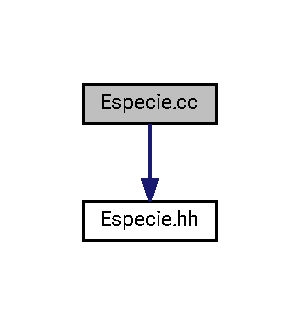
\includegraphics[width=144pt]{_especie_8cc__incl}
\end{center}
\end{figure}


\subsection{Descripció Detallada}
Codi de la classe \hyperlink{class_especie}{Especie}. 


\hypertarget{_especie_8hh}{}\section{Referència del Fitxer Especie.\+hh}
\label{_especie_8hh}\index{Especie.\+hh@{Especie.\+hh}}


Especificació de la clase \hyperlink{class_especie}{Especie}.  


\subsection*{Classes}
\begin{DoxyCompactItemize}
\item 
class \hyperlink{class_especie}{Especie}
\begin{DoxyCompactList}\small\item\em Representa una espècie. \end{DoxyCompactList}\end{DoxyCompactItemize}


\subsection{Descripció Detallada}
Especificació de la clase \hyperlink{class_especie}{Especie}. 


\hypertarget{_individu_8cc}{}\section{Referència del Fitxer Individu.\+cc}
\label{_individu_8cc}\index{Individu.\+cc@{Individu.\+cc}}


Codi de la classe \hyperlink{class_individu}{Individu}.  


Inclou el graf de dependències per a Individu.\+cc\+:\nopagebreak
\begin{figure}[H]
\begin{center}
\leavevmode
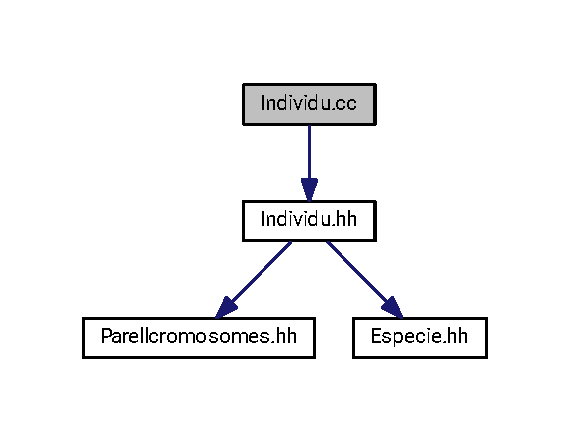
\includegraphics[width=274pt]{_individu_8cc__incl}
\end{center}
\end{figure}


\subsection{Descripció Detallada}
Codi de la classe \hyperlink{class_individu}{Individu}. 


\hypertarget{_individu_8hh}{}\section{Referència del Fitxer Individu.\+hh}
\label{_individu_8hh}\index{Individu.\+hh@{Individu.\+hh}}


Especificació de la clase \hyperlink{class_individu}{Individu}.  


Inclou el graf de dependències per a Individu.\+hh\+:\nopagebreak
\begin{figure}[H]
\begin{center}
\leavevmode
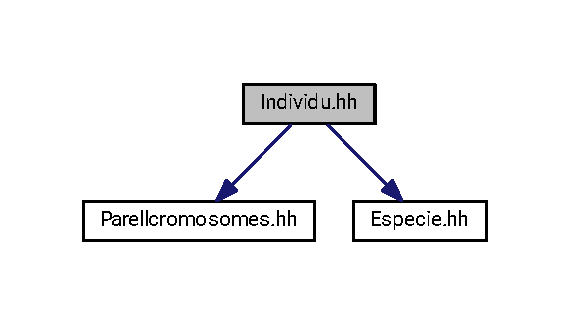
\includegraphics[width=274pt]{_individu_8hh__incl}
\end{center}
\end{figure}
\subsection*{Classes}
\begin{DoxyCompactItemize}
\item 
class \hyperlink{class_individu}{Individu}
\begin{DoxyCompactList}\small\item\em Representa un individu. \end{DoxyCompactList}\end{DoxyCompactItemize}


\subsection{Descripció Detallada}
Especificació de la clase \hyperlink{class_individu}{Individu}. 


\hypertarget{_parellcromosomes_8cc}{}\section{Referència del Fitxer Parellcromosomes.\+cc}
\label{_parellcromosomes_8cc}\index{Parellcromosomes.\+cc@{Parellcromosomes.\+cc}}


Codi de la classe Parellcromosomes.  


Inclou el graf de dependències per a Parellcromosomes.\+cc\+:\nopagebreak
\begin{figure}[H]
\begin{center}
\leavevmode
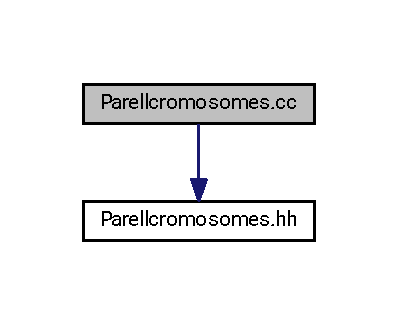
\includegraphics[width=191pt]{_parellcromosomes_8cc__incl}
\end{center}
\end{figure}


\subsection{Descripció Detallada}
Codi de la classe Parellcromosomes. 


\hypertarget{_parellcromosomes_8hh}{}\section{Referència del Fitxer Parellcromosomes.\+hh}
\label{_parellcromosomes_8hh}\index{Parellcromosomes.\+hh@{Parellcromosomes.\+hh}}


Especificació de la clase Parellcromosomes.  


\subsection*{Classes}
\begin{DoxyCompactItemize}
\item 
class \hyperlink{class_parell__cromosomes}{Parell\+\_\+cromosomes}
\begin{DoxyCompactList}\small\item\em Representa un parell de cromosomes. \end{DoxyCompactList}\end{DoxyCompactItemize}


\subsection{Descripció Detallada}
Especificació de la clase Parellcromosomes. 


\hypertarget{_poblacio_8cc}{}\section{Referència del Fitxer Poblacio.\+cc}
\label{_poblacio_8cc}\index{Poblacio.\+cc@{Poblacio.\+cc}}


Codi de la classe \hyperlink{class_poblacio}{Poblacio}.  


Inclou el graf de dependències per a Poblacio.\+cc\+:\nopagebreak
\begin{figure}[H]
\begin{center}
\leavevmode
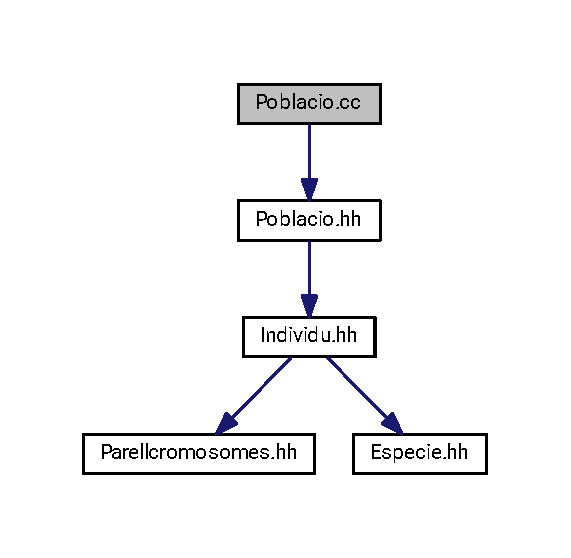
\includegraphics[width=274pt]{_poblacio_8cc__incl}
\end{center}
\end{figure}


\subsection{Descripció Detallada}
Codi de la classe \hyperlink{class_poblacio}{Poblacio}. 


\hypertarget{_poblacio_8hh}{}\section{Referència del Fitxer Poblacio.\+hh}
\label{_poblacio_8hh}\index{Poblacio.\+hh@{Poblacio.\+hh}}


Especificació de la clase \hyperlink{class_poblacio}{Poblacio}.  


Inclou el graf de dependències per a Poblacio.\+hh\+:\nopagebreak
\begin{figure}[H]
\begin{center}
\leavevmode
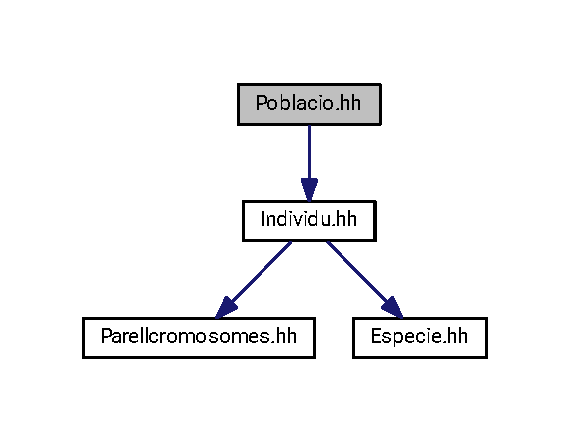
\includegraphics[width=274pt]{_poblacio_8hh__incl}
\end{center}
\end{figure}
\subsection*{Classes}
\begin{DoxyCompactItemize}
\item 
class \hyperlink{class_poblacio}{Poblacio}
\begin{DoxyCompactList}\small\item\em Representa una població. \end{DoxyCompactList}\end{DoxyCompactItemize}


\subsection{Descripció Detallada}
Especificació de la clase \hyperlink{class_poblacio}{Poblacio}. 


\hypertarget{program_8cc}{}\section{Referència del Fitxer program.\+cc}
\label{program_8cc}\index{program.\+cc@{program.\+cc}}


Programa principal de la pràctica {\itshape {\bfseries Experiments genètics en un laboratori}}.  


Inclou el graf de dependències per a program.\+cc\+:\nopagebreak
\begin{figure}[H]
\begin{center}
\leavevmode
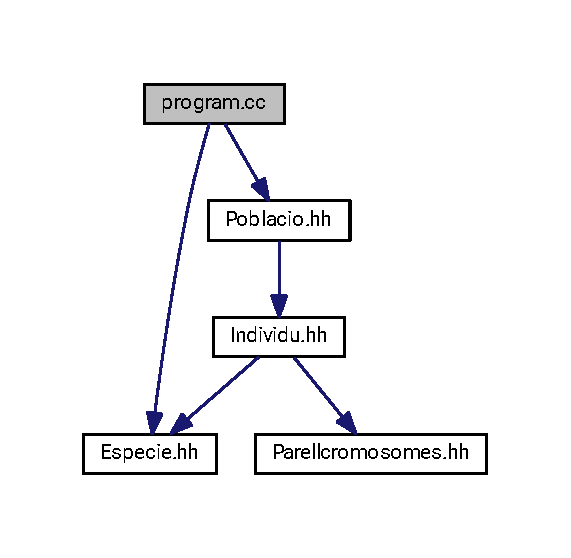
\includegraphics[width=274pt]{program_8cc__incl}
\end{center}
\end{figure}
\subsection*{Funcions}
\begin{DoxyCompactItemize}
\item 
int \hyperlink{program_8cc_ae66f6b31b5ad750f1fe042a706a4e3d4}{main} ()
\begin{DoxyCompactList}\small\item\em Programa principal de la pràctica {\itshape Experiments genètics en un laboratori}. \end{DoxyCompactList}\end{DoxyCompactItemize}


\subsection{Descripció Detallada}
Programa principal de la pràctica {\itshape {\bfseries Experiments genètics en un laboratori}}. 



\subsection{Documentació de les Funcions}
\index{program.\+cc@{program.\+cc}!main@{main}}
\index{main@{main}!program.\+cc@{program.\+cc}}
\subsubsection[{\texorpdfstring{main()}{main()}}]{\setlength{\rightskip}{0pt plus 5cm}int main (
\begin{DoxyParamCaption}
{}
\end{DoxyParamCaption}
)}\hypertarget{program_8cc_ae66f6b31b5ad750f1fe042a706a4e3d4}{}\label{program_8cc_ae66f6b31b5ad750f1fe042a706a4e3d4}


Programa principal de la pràctica {\itshape Experiments genètics en un laboratori}. 



Definició a la línia 28 del fitxer program.\+cc.


\begin{DoxyCode}
28           \{
29 
30     \hyperlink{class_especie}{Especie} esp;
31 
32     esp.\hyperlink{class_especie_a5c424f7536e2e5fcb7e7e5452ab24ff7}{establir\_genetica}();
33 
34     \hyperlink{class_poblacio}{Poblacio} poble;
35     
36     poble.\hyperlink{class_poblacio_a8757ef86688a1e2c25d9264aea934a28}{llegir\_inicials}(esp);
37     
38     \textcolor{keywordtype}{string} accio;
39 
40     \textcolor{keywordflow}{while} (cin >> accio and accio != \textcolor{stringliteral}{"acabar"})\{
41         
42         \textcolor{keywordflow}{if} (accio == \textcolor{stringliteral}{"anadir\_individuo"})\{
43             poble.\hyperlink{class_poblacio_a29df411fde89d37a05fb705e1cc3dd8b}{llegir}(esp);
44         \}
45 
46         \textcolor{keywordflow}{else} \textcolor{keywordflow}{if} (accio == \textcolor{stringliteral}{"reproduccion\_sexual"})\{
47             \textcolor{keywordtype}{string} mare, pare, fill;
48             cin >> mare >> pare >> fill;
49             
50             poble.\hyperlink{class_poblacio_a9e31f2e6394618bc130280322cb24fbf}{reproduir}(pare, mare, fill, esp);
51             
52         \}
53         
54         \textcolor{keywordflow}{else} \textcolor{keywordflow}{if} (accio == \textcolor{stringliteral}{"escribir\_arbol\_genealogico"})\{
55             \textcolor{keywordtype}{string} nom;
56             cin >> nom;
57             poble.\hyperlink{class_poblacio_a82a6f322f03527ab4273223f351c1036}{escriure\_arbre\_genealogic}(nom);
58         \}
59 
60         \textcolor{keywordflow}{else} \textcolor{keywordflow}{if} (accio == \textcolor{stringliteral}{"completar\_arbol\_genealogico"})\{
61             poble.\hyperlink{class_poblacio_abe25acd8c2ce02a747ab79f26cc74f11}{completar\_arbre}();
62         \}
63 
64         \textcolor{keywordflow}{else} \textcolor{keywordflow}{if} (accio == \textcolor{stringliteral}{"escribir\_poblacion"})\{
65             poble.\hyperlink{class_poblacio_acef5af456368a81c4f3be0bd44841bf1}{escriure\_poblacio}();
66         \}
67 
68         \textcolor{keywordflow}{else} \textcolor{keywordflow}{if} (accio == \textcolor{stringliteral}{"escribir\_genotipo"})\{
69             \textcolor{keywordtype}{string} nom;
70             cin >> nom;
71             
72             cout << \textcolor{stringliteral}{"escribir\_genotipo "} << nom << endl;
73             
74             \textcolor{keywordflow}{if} (poble.\hyperlink{class_poblacio_ac32cb311f3b283b82adf3d0b7d82fbcc}{existeix\_individu}(nom)) poble.
      \hyperlink{class_poblacio_a0574c7b81e2b8329fb2ffcd0b4365a98}{consultar\_individu}(nom).\hyperlink{class_individu_a66e02b3d1a7e327ffb152c1e6193407a}{escriure\_genotip}();
75             
76             \textcolor{keywordflow}{else} cout << \textcolor{stringliteral}{"  error"} << endl;
77         \}
78     \}
79     
80     cout << \textcolor{stringliteral}{"acabar"} << endl;
81 
82     
83     
84 \}
\end{DoxyCode}

%--- End generated contents ---

% Index
\backmatter
\newpage
\phantomsection
\clearemptydoublepage
\addcontentsline{toc}{chapter}{Índex}
\printindex

\end{document}
